% =====================================================================
% Comprehensive architecture study — Recurrent Vision Transformers as
% models of primate visual attention. Internal progress thesis.
% Build:  pdflatex main ; bibtex main ; pdflatex main ; pdflatex main
% (PATH=$PATH:/Library/TeX/texbin). Minimal-TeX safe: no siunitx/authblk. TikZ (core
% libraries only — no shadows.blend) is used for the architecture atlas (App.~A).
% =====================================================================
\documentclass[11pt]{report}
\usepackage[utf8]{inputenc}
\usepackage[T1]{fontenc}
\usepackage{lmodern}
\usepackage[a4paper,margin=1in]{geometry}
\usepackage{amsmath,amssymb,amsthm,mathtools}
\usepackage{graphicx}
\usepackage{booktabs}
\usepackage{longtable}
\usepackage{array}
\usepackage[dvipsnames]{xcolor}
\usepackage{tikz}
\usepackage{caption}
\captionsetup{labelfont=bf,textfont=small,labelsep=period}
\usepackage[round]{natbib}
\bibliographystyle{plainnat}
\usepackage[colorlinks=true,allcolors=blue!45!black]{hyperref}
\graphicspath{{figures/}{figures/atlas/}{figures/atlas_t29/}{figures/jepa/}}
% Shared TikZ style for the architecture atlas. \input by the thesis preamble AND by each
% standalone compile-test wrapper, so diagrams render identically in both. Core libraries
% only (shadows.blend is unavailable in this TeX install).
\usetikzlibrary{positioning,arrows.meta,calc,fit,backgrounds,shapes.geometric,shapes.misc,decorations.pathreplacing}
\tikzset{
  % ---- node roles (colour = function; shared by every diagram) -------------------------
  blk/.style   ={draw,rounded corners=2.2pt,minimum height=8.5mm,minimum width=15mm,align=center,font=\scriptsize,line width=.6pt},
  vae/.style   ={blk,fill=RoyalBlue!10,draw=RoyalBlue!55},   % VAE / front-end (frozen)
  tok/.style   ={blk,fill=RoyalBlue!4,draw=RoyalBlue!40,minimum width=9mm},   % token tensor
  attn/.style  ={blk,fill=teal!12,draw=teal!60},             % attention / ViT block
  mem/.style   ={blk,fill=BurntOrange!16,draw=BurntOrange!70},% xLSTM working memory
  cb/.style    ={blk,fill=Goldenrod!22,draw=Goldenrod!80},   % codebook / learnable table
  head/.style  ={blk,fill=Orchid!16,draw=Orchid!70},         % actor / critic heads
  op/.style    ={draw,circle,inner sep=0pt,minimum size=4.6mm,fill=gray!10,font=\scriptsize,line width=.5pt},
  % ---- edges (style = semantics) -------------------------------------------------------
  flow/.style  ={->,>=Latex,line width=.75pt,draw=black!75},          % forward dataflow
  fb/.style    ={->,>=Latex,line width=.75pt,dashed,draw=Red!65},     % recurrent feedback (prev frame)
  qkv/.style   ={->,>=Latex,line width=.55pt,draw=black!55},          % into Q/K/V construction
  lbl/.style   ={font=\scriptsize\itshape,text=black!70,align=center},
}
% colour legend strip — every atlas figure can drop this in for a consistent key
\newcommand{\archlegend}{%
  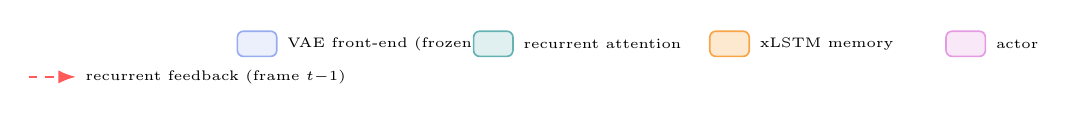
\begin{tikzpicture}[baseline]
    \foreach \s/\t [count=\i] in {vae/VAE front-end (frozen),attn/recurrent attention,mem/xLSTM memory,head/actor\,/\,critic} {
      \node[\s,minimum width=5mm,minimum height=3.2mm] (L\i) at (\i*3.0,0) {};
      \node[anchor=west,font=\tiny] at (L\i.east) {\t};
    }
    \draw[fb] (0.1,-0.42)--(0.7,-0.42); \node[anchor=west,font=\tiny] at (0.7,-0.42){recurrent feedback (frame $t{-}1$)};
  \end{tikzpicture}}
   % shared TikZ styles for the architecture atlas (App.~A)

% notation shorthands
\newcommand{\X}{\mathbf{X}}
\newcommand{\Hone}{\mathbf{H}_1}
\newcommand{\Htwo}{\mathbf{H}_2}
\newcommand{\Zmu}{\mathbf{Z}_\mu}
\newcommand{\Zq}{\mathbf{Z}_q}
\newcommand{\Rsq}{R^{2}}
\newcommand{\dmem}{d_{\text{mem}}}
\newcommand{\oflat}{\mathbf{o}_{\text{flat,2}}}
\newcommand{\code}[1]{\texttt{#1}}

\title{\bfseries Recurrent Vision Transformers as Models of Primate Visual
Attention:\\[4pt] A Comprehensive Architecture Study\\[10pt]
\large Internal progress report}
\author{RViT architecture program\\\small Morgan, Albanna \& Herman}
\date{Compiled \today}

\begin{document}
\maketitle

\begin{abstract}
\noindent
This report consolidates everything the architecture program has learned about
building a recurrent vision transformer (RViT) that reproduces the behavioural and
neural signatures of primate covert spatial attention while learning end-to-end from
sparse reward. Across roughly thirty network variants and two task horizons we isolate
a small number of load-bearing findings. \textbf{(1) Perception is the bottleneck on the
short (seven-step) task.} Sparse reward cannot teach the front-end to represent
orientation: a reconstruction-pretrained VAE encoder lifts the linear decodability of
Gabor orientation from $\Rsq=0.24$ to $\Rsq=0.97$, and with that single change the exact
paper network learns the task on the first attempt. \textbf{(2) The horizon governs which
strategy is viable.} On the long task a weak front-end suffices because the change
persists long enough to be detected by slow temporal integration (``optic flow''); the
short task removes that escape hatch and forces accurate single-frame perception.
\textbf{(3) Coupling between the policy and value pathways is a precondition for
learning,} not an optimisation: cutting the shared recurrent memory collapses an
otherwise identical split-pathway model to chance. \textbf{(4) The working model reproduces
the paper's core behavioural figures} --- a reliability-scaled psychometric cueing benefit
($+1.5^\circ\!\to\!+7.5^\circ$ across $25\%\!\to\!100\%$ validity) and a causal
attention-to-sensitivity link ($+8.5\%/-8.0\%$ from biasing attention toward/away from a
change). \textbf{(5) The cueing effect is memory-driven rather than attention-driven, across an
entire matched family:} in the multiplicative-gated model the cue and its validity are held
in recurrent memory ($100\%$ decodable) while the attention map stays change-locked, and a
matched family of six attention/memory wirings (multiplicative, dual-head, two-LSTM,
cross-attention, dual-memory, and a failed affine modulation) confirms that \emph{no} working
variant orients attention to the cue on the short task --- two of them attend markedly
\emph{away} from the cued image location. The same sweep names the network to carry forward:
the two-LSTM multiplicative form is the best detector. We close with that recommendation for
the empirical manuscript, a proposed task battery (VDA, set-size, Luo \& Maunsell, Krauzlis),
and a staged research plan.
\end{abstract}

\tableofcontents

\chapter{Introduction}
\label{ch:intro}

\section{The program and its goal}
The long-run objective of this program is a single neural-network architecture that (i)
learns covert visual attention end-to-end from sparse, animal-like reward, (ii)
reproduces the behavioural and neural signatures of primate spatial attention, and (iii)
\emph{generalises} across the standard battery of non-human-primate (NHP) attention tasks
rather than being tuned to one. We are not merely fitting a curve; we are searching for
the most neuro-inspired wiring that makes attentive behaviour \emph{emerge} from the
combination of a learnable priority computation, a capacity-limited working memory, and a
reward signal --- and that, having emerged, exposes an interpretable and causally
manipulable internal attention signal.

The published manuscript this program supports, \emph{``A recurrent vision transformer
shows signatures of primate visual attention''} (Morgan, Albanna \& Herman), establishes
the empirical claim on the canonical four-stimulus, validity-driven, uniform-reward task.
This report is the architecture study that sits behind that manuscript: it records what
we tried, what worked, what failed, and --- most importantly --- \emph{why}, so that the
choice of network to carry forward is grounded in evidence rather than habit.

\section{The model in one paragraph}
The recurrent vision transformer parses each video frame into a small set of spatial
patch tokens, runs a \emph{recurrent} self-attention block in which the attention is
computed jointly from the current image and the contents of a per-patch working memory,
writes that memory with a spatial long short-term memory (LSTM) cell, and reads the
memory with a distributional actor--critic head trained by reinforcement learning. The
defining property is the recurrence of attention: because the attention at frame $t$
depends on memory accumulated from previous frames, a cue shown briefly and then removed
can be maintained and used to bias later processing. Every architectural decision in this
report is, at bottom, a decision about \emph{how} the image and the memory combine to form
attention, and \emph{which} internal state the decision is read from.

\section{Scope of the evidence}
The findings synthesised here rest on roughly thirty network variants trained on two task
horizons, plus a clean-room reproduction of the exact published network. The variants
span memory-as-tokens self-attention, cross-attention over memory, multiplicative
(FiLM-style) gain modulation, vector-quantised codebook attention, predictive-coding and
energy-modulation front-ends, split actor/critic pathways with and without cross-talk,
fast-weight (hypernetwork) attention, and several novel dual-memory wirings. Two
front-ends (raw-pixel and a reconstruction-pretrained VAE) and two reinforcement-learning
horizons (a seven-step fixed-onset task and a twenty-nine-step random-onset task) complete
the design space. The reinforcement-learning machinery --- prioritised episode replay, a
maximum-a-posteriori-policy-optimisation actor loss, and a distributional quantile critic
--- is held essentially constant so that architectural comparisons are clean.

\section{Contributions and structure}
The contributions, each developed in its own chapter, are:
\begin{enumerate}
\item \textbf{Perception is the bottleneck on the short task} (Chapter~\ref{ch:perception}).
A reconstruction-pretrained VAE front-end is necessary and nearly sufficient to make the
exact paper network learn the seven-step task; a front-end trained from reward alone never
learns to represent orientation and the agent collapses to pressing at the deadline.
\item \textbf{The horizon decides which strategy is viable} (Chapter~\ref{ch:horizon}).
The long task tolerates a weak front-end because the change can be integrated over many
frames; the short task does not, which is why the VAE matters on one and not the other.
\item \textbf{Coupling is a precondition for learning} (Chapter~\ref{ch:crosstalk}).
Severing the shared memory between the policy and value streams collapses an otherwise
identical model to chance --- shared memory is load-bearing, not cosmetic.
\item \textbf{The working network reproduces the paper's behaviour}
(Chapter~\ref{ch:deepdive}): the reliability-scaled psychometric cueing benefit and the
causal attention-to-sensitivity link both replicate cleanly.
\item \textbf{Cueing can be carried by memory rather than attention}
(Chapter~\ref{ch:attention}): a mechanistic dissociation that reframes how we read the
attention maps and motivates a family of follow-up wirings.
\end{enumerate}
The remaining chapters catalogue the full architecture zoo
(Chapter~\ref{ch:zoo}), survey the reinforcement-learning harness and its variations
(Chapters~\ref{ch:harness} and \ref{ch:harnessvar}), and close with an architecture
recommendation (Chapter~\ref{ch:recommendation}), a proposed task battery
(Chapter~\ref{ch:experiments}), a research plan (Chapter~\ref{ch:plan}), and a one-page
summary of the actionable findings (Chapter~\ref{ch:findings}).

\section{A note on terminology}
Throughout, we call the two recurrent streams of the split-pathway models the
\emph{priority} ($\mu$) pathway, which feeds the actor and the decision of \emph{when} to
declare a change, and the \emph{value} ($q$) pathway, which feeds the critic. We avoid the
labels ``salience'' and ``top-down'' because the priority/commitment areas of the brain
(LIP, FEF, SC) are each a single priority map rather than an actor/critic pair; the
$\mu$/$q$ split is a computational decomposition, and we are careful in
Chapter~\ref{ch:recommendation} about the limits of mapping it onto anatomy.

\chapter{The task and its environments}
\label{ch:task}

\section{The canonical cued change-detection task}
The base environment is a spatially cued orientation-change-detection task built to
reproduce the essential structure of primate covert-attention experiments. Each trial is
a short video of $50\times50$ grayscale frames. The canonical (paper) timeline is
\textbf{seven frames}:
\begin{itemize}
\item $t=0$: black screen.
\item $t=1$: a spatial \emph{cue} appears at one stimulus location --- top-left ($S_1$) or
bottom-right ($S_4$). The cue is a disc whose surrounding ring is completed in proportion
to the cue's \emph{validity} (the probability that, on a change trial, the change will
occur at the cued location): $25\%$, $50\%$, $75\%$, or $100\%$.
\item $t=2$: black screen (the cue is removed; its information must now be held in memory).
\item $t=3,4$: four Gabor-like stimuli appear, one per quadrant ($S_1$ top-left, $S_2$
bottom-left, $S_3$ top-right, $S_4$ bottom-right), at random orientations at least
$45^\circ$ apart, with per-frame orientation ``wobble''.
\item $t=5$: on half of trials (\emph{change trials}) one stimulus's orientation steps by
$\Delta$ degrees; on the other half nothing changes. The change persists to $t=6$.
\item $t=6$: final frame.
\end{itemize}
At every frame the agent chooses \emph{wait} or \emph{declare change}. Declaring ends the
trial. A correct declaration at $t\geq5$ earns reward $1$; waiting out a no-change trial to
$t=6$ also earns $1$; everything else earns $0$. The two errors are therefore misses
(failing to declare a real change) and false alarms (declaring on a no-change trial or
declaring prematurely).

\section{Difficulty control}
Difficulty is set by two knobs. \textbf{Orientation noise} $\sigma$ adds frame-to-frame
jitter $\delta_{it}\sim\mathcal N(0,\sigma)$ to each stimulus orientation; $\sigma=5$ in
the canonical task. The \textbf{change magnitude} $\Delta$ is drawn per change trial from
$\mathcal U(-k,k)$, with $k$ starting at $65^\circ$ and shrinking by a curriculum (factor
$0.9$ each time rolling accuracy exceeds $0.85$, floor $8^\circ$) so the task hardens as
the agent improves. For psychometric analysis we override $\Delta$ to fixed magnitudes and
freeze the curriculum, exactly as one would titrate difficulty in an animal.

\section{Why the seven-step task is hard for reinforcement learning}
The short horizon makes the task deceptively difficult to \emph{learn} even though it is
easy to \emph{solve} (a scripted ``wait until the change is visible, then press'' policy
scores $1.000$). Two degenerate strategies sit at $0.5$ accuracy and act as attractors:
\emph{always-wait} (correct on every no-change trial, misses every change) and
\emph{always-press-at-the-deadline} (catches every change, false-alarms every no-change).
Because the change persists for only two frames, the reward-bearing ``correct press''
window is narrow, so the discriminating policy is hard to discover by exploration, and the
policy entropy collapses before discovery. This is the central learning obstacle the
perception and architecture findings of later chapters are really about.

\section{The task battery}
The same environment generalises to the standard NHP battery by editing the reward branch
and the cue, which is how James proposes to broaden the empirical paper's scope. The
implemented and planned variants are:
\begin{itemize}
\item \textbf{\code{validity4}} --- the canonical four-stimulus, uniform-reward,
validity-driven task above. The workhorse of this report.
\item \textbf{\code{vda4}} --- value-cue variant: the cue colour (red/green/blue) sets the
reward magnitude ($5/3/1$), so behaviour can be read for value direction as well as
spatial cueing.
\item \textbf{\code{setsize\{2,4,9\}}} --- set-size manipulation; the nine-stimulus
($3\times3$) version with five validity levels (including an uninformative $0$) tests
whether the cueing benefit \emph{grows} with set size, the bridge to the normative
set-size/accidental-hit theory (Paper B).
\item \textbf{distractor} (the \code{v7}/\code{v11\_part5} env) --- the cue selects a
\emph{side}; the uncued side independently changes with probability $0.5$ and must be
ignored (pressing on it is a false alarm). Tests genuine selection against a competitor.
\item \textbf{\code{luo\_maunsell}} --- reward-structure manipulation (sensitivity vs.
criterion sessions) after Luo \& Maunsell (2018).
\item \textbf{\code{krauzlis}} --- attend/ignore manipulation after Krauzlis and
colleagues, where an uncued change must be actively ignored.
\end{itemize}
All variants share the clean \code{ChangeDetectionEnv} interface: \code{reset} draws the
cue, validity, and change; \code{step} exposes the two actions and the reward branch. This
uniformity is what makes ``train one architecture across the whole battery'' a tractable
research goal rather than a per-task engineering effort.

\section{The long-horizon variant}
A twenty-nine-step variant (\code{T}=29, change onset drawn uniformly in $[11,25]$) is used
throughout the architecture history. It is the same task with a much longer post-change
window, and as Chapter~\ref{ch:horizon} shows, that single difference --- the length of the
window over which a change can be integrated --- explains most of the otherwise puzzling
discrepancies between the two horizons.

\chapter{The model architecture}
\label{ch:model}

The recurrent vision transformer has four stages: a patch front-end, a recurrent
self-attention block, a spatial recurrent memory, and an actor--critic readout. This
chapter gives the canonical (paper) form of each; later chapters vary one stage at a time.

\section{Patch front-end}
Each $50\times50$ frame is divided into four $25\times25$ quadrants. In the canonical
network each quadrant is encoded by the encoder of a variational autoencoder (VAE) up to
its second flattened layer, a $128$-dimensional feature $\oflat$ (the paper feeds the ViT
this layer, not the stochastic latent). Per-patch positional and per-frame temporal
one-hot codes are concatenated, giving a $140$-dimensional token, and the four tokens form
$\X^{(t)}\in\mathbb R^{4\times140}$. The role of the VAE --- and the consequence of
training it from reward versus from reconstruction --- is the subject of
Chapter~\ref{ch:perception}.

\section{Recurrent multiplicative self-attention}
The canonical attention is single-head and \emph{multiplicatively gated} by memory. With
the previous-frame memory $\Hone^{(t-1)}\in\mathbb R^{4\times\dmem}$ ($\dmem=1024$),
\begin{align}
\mathbf Q &= (\X\,\mathbf W_{XQ})\odot(\Hone\,\mathbf W_{HQ}), &
\mathbf K &= (\X\,\mathbf W_{XK})\odot(\Hone\,\mathbf W_{HK}), &
\mathbf V &= (\X\,\mathbf W_{XV})\odot(\Hone\,\mathbf W_{HV}),
\label{eq:mult}
\end{align}
with $\mathbf W_{X\cdot}\in\mathbb R^{140\times140}$, $\mathbf W_{H\cdot}\in\mathbb
R^{1024\times140}$, $\odot$ the Hadamard product, and the attention
\begin{equation}
\mathbf V_{\text{filt}}=\mathrm{softmax}(\mathbf Q\mathbf K^\top)\mathbf V,\qquad
\mathbf Z^{(t)}=\X^{(t)}+\mathbf V_{\text{filt}}\in\mathbb R^{4\times140}.
\label{eq:z}
\end{equation}
The multiplicative form is the program's neuro-motivated gain-modulation: memory does not
add to the image, it \emph{scales} the bottom-up query/key/value projections. As
Chapter~\ref{ch:attention} documents, this exact form has an important consequence ---
when memory is uninformative the gate is near zero and the attention is uniform --- which
is at the heart of the attention/memory dissociation. The cross-attention and FiLM
variants replace Eq.~\eqref{eq:mult} with, respectively, $\mathbf K,\mathbf V$ formed by
concatenating image and memory tokens, and a $(1+\Hone\mathbf W_{H})$ identity-floored
gate.

\section{Spatial recurrent memory}
The percept $\mathbf Z$ writes a per-patch memory through an exponential-gated spatial
LSTM (an adaptation of the xLSTM), maintained independently per patch so that
self-attention is the only route by which spatial locations exchange information:
\begin{align*}
\tilde{\mathbf I}&=\mathbf Z\mathbf W_i+\mathbf H\mathbf R_i, &
\tilde{\mathbf F}&=\mathbf Z\mathbf W_f+\mathbf H\mathbf R_f, &
\tilde{\mathbf O}&=\mathbf Z\mathbf W_o+\mathbf H\mathbf R_o, &
\tilde{\mathbf U}&=\mathbf Z\mathbf W_u+\mathbf H\mathbf R_z,\\
\mathbf M&=\max(\tilde{\mathbf F}+\mathbf M',\tilde{\mathbf I}), &
\mathbf I&=e^{\tilde{\mathbf I}-\mathbf M}, &
\mathbf F&=e^{\tilde{\mathbf F}+\mathbf M'-\mathbf M}, &
\mathbf O&=\sigma(\tilde{\mathbf O}),
\end{align*}
\[
\mathbf N=\mathbf F\odot\mathbf N'+\mathbf I,\quad
\mathbf C=\mathbf C'\odot\mathbf F+\tanh(\tilde{\mathbf U})\odot\mathbf I,\quad
\mathbf H=\mathbf O\odot(\mathbf C/\mathbf N),
\]
with $\dmem=1024$, $\mathbf W_x\in\mathbb R^{140\times1024}$, $\mathbf
R_x\in\mathbb R^{1024\times1024}$, and the stabiliser/normaliser states $\mathbf M,\mathbf
N$. The memory is the agent's working memory: it carries the cue and the accumulating
evidence across the blank interval.

\section{Actor--critic readout}
The four-patch structure is retained through attention and memory but \emph{flattened} at
the reinforcement-learning agent: the readout is $\mathbf H'\in\mathbb R^{4096}$. A
four-layer feed-forward actor maps $\mathbf H'$ to a two-way policy (wait / declare); a
distributional critic maps $\mathbf H'$ to a value distribution. Which internal state is
read --- the flattened memory $\mathbf H$ (canonical) versus the attention output
$\mathbf Z$ (the cross-talk and codebook variants) --- is itself an architectural variable
that, we find, changes the phenotype.

\begin{table}[t]
\centering
\caption{Components of the canonical recurrent vision transformer and the axes along which
the architecture zoo varies them.}
\label{tab:components}
\small
\begin{tabular}{p{2.6cm}p{4.6cm}p{5.4cm}}
\toprule
Stage & Canonical form & Variation axis explored \\
\midrule
Front-end & VAE encoder $\to\oflat$ (128-d), 4 tokens & raw-pixel vs.\ conv vs.\ frozen
VAE; 4 vs.\ 100 tokens \\
Attention & multiplicative gate, single head & cross-attention, FiLM $(1{+}\cdot)$,
fast-weights, codebook, dual-head \\
Feedback source & memory $\Hone$ scales Q/K/V & memory as keys/values; memory generates
weights; memory as queries \\
Memory & one xLSTM, $\dmem{=}1024$ & two LSTMs (feedback vs.\ decision); parallel vs.\
stacked; LSTM vs.\ vanilla \\
Readout & flattened $\mathbf H$ (4096) & read $\mathbf Z$; split $\mu/q$; codebook
selection \\
\bottomrule
\end{tabular}
\end{table}

\chapter{The reinforcement-learning harness}
\label{ch:harness}

The agent learns purely from the sparse task reward; there is no reconstruction or
auxiliary loss on the recurrent network (the VAE, when used, is pretrained separately and
frozen). The harness has been held essentially constant across architectures so that
comparisons are clean, and it is itself one of the program's hard-won results: a stable
recipe for training a bootstrapped recurrent actor--critic on a task with a deceptive
$0.5$ accuracy floor.

\section{Actor: PAC (maximum-a-posteriori policy optimisation $+$ behaviour cloning)}
The actor loss replaces the clipped PPO surrogate with the PAC objective. For the discrete
action set the maximum-a-posteriori-policy-optimisation E-step is closed form,
\begin{equation}
q(a\mid s)=\mathrm{softmax}_a\!\big[\log\pi_{\theta'}(a\mid s)+\bar Q_{\theta'}(s,a)/\eta\big],
\end{equation}
where $\theta'$ is a time-lagged target network, $\bar Q$ is the critic's mean over the
value distribution, and $\eta$ is a temperature. The M-step plus a behaviour-cloning term
gives
\[
\mathcal L_{\text{actor}}=(1-\alpha)\Big(-\textstyle\sum_a q(a\mid s)\log\pi_\theta(a\mid s)\Big)
+\alpha\big(-\log\pi_\theta(a_t\mid s)\big),
\]
with $\eta=0.1$, $\alpha=0.1$. The critic's value drives the actor \emph{directly}; there
is no generalised-advantage estimation.

\section{Critic: distributional quantile regression}
The critic is a distributional QR-DQN critic: it predicts a set of value quantiles and is
trained with the quantile-Huber loss against the one-step distributional temporal-
difference target $r_t+\gamma\,\mathbf V_{\text{dist}}(s_{t+1})(1-d_t)$. The published
network used a $15$-bin categorical critic; in the reproduction we use $5$--$15$ quantiles.
The number of ``particles'' is a deliberate knob (Chapter~\ref{ch:harnessvar}).

\section{Prioritised episode replay}
Fresh on-policy episodes are augmented with replay episodes drawn at episode granularity
$\propto$ priority$^{\alpha}$, priority being the mean per-step quantile-Huber error,
with importance-sampling weights annealed over training. Episode-level replay is essential
on this task: the discriminating ``correct press'' events are rare, and replay keeps them
in the gradient long enough to be learned.

\section{Target network: hard-copy versus EMA}
The target network $\theta'$ supplies both the critic's bootstrap target and the actor's
E-step reference policy. Two update rules are available: a periodic hard copy ($\theta'\!
\leftarrow\!\theta$ every $N$ optimiser steps, the form that produced the original working
checkpoints) and an exponential moving average ($\theta'\!\leftarrow\!d\,\theta'+(1-d)
\theta$ each iteration). The EMA form was added during the reproduction; whether it is
load-bearing is one of the open A/B questions of Chapter~\ref{ch:harnessvar}.

\section{Burn-in}
For the first $\sim\!20$ iterations the agent is forced to wait, training only the critic
on full-length episodes so the value function and recurrent representation warm up on clean
trajectories before the policy acts. This is the descendant of the program's earlier
reconstruction-pretrain phase and materially reduces the early collapse to premature
pressing.

\section{What the harness taught us}
Three lessons recur in the history. First, \textbf{always-wait is a stable harbor}: a
bootstrapped actor on this task will retreat to the safe action that never incurs a
false-alarm penalty unless exploration is actively maintained. Second, \textbf{the target
network is the main stabiliser}: a time-lagged reference for both the critic target and
the E-step reference policy is what keeps the bootstrap from chasing its own tail. Third,
\textbf{a degenerate $0.5$ optimum has two faces} (always-wait and always-press-at-deadline)
and which one a run falls into is seed-dependent --- both are collapses, and escaping them
is a perception/exploration problem, not a critic problem (the critic learns the $0.5$
value perfectly well in both).

\chapter{Finding I --- perception is the bottleneck}
\label{ch:perception}

The single most consequential result of the reproduction is that, on the seven-step task,
the obstacle to learning is not the reinforcement-learning objective, the attention
mechanism, or the memory --- it is \emph{perception}. A front-end trained from reward alone
never learns to represent orientation, and the agent therefore cannot see the change it is
asked to report.

\section{The collapse}
The exact published network, trained end-to-end for the full $150{,}000$ episodes with the
VAE encoder learned from reward, does not reproduce the task. It converges to
\emph{always-press-at-the-deadline}: it presses at frame $5$ (the first frame a change
could appear) on every trial, scoring hit rate $1.000$ on change trials and false-alarm
rate $1.000$ on no-change trials, for an overall accuracy of $0.515$ and a reaction time
pinned at exactly five frames. It has learned the \emph{timing} of the change window but
not the \emph{discrimination} of change from no-change.

\section{The diagnosis}
Why can it not discriminate? Because to detect an orientation change one must represent
orientation, and the from-scratch front-end does not. We probed this directly: render
single Gabor patches at known orientations, encode them through the trained front-end's
$\oflat$ layer, and fit a linear decoder for the (circular) orientation. The result is
decisive (Fig.~\ref{fig:vaer2}):
\[
\Rsq_{\text{from-scratch}}=0.24,\qquad \Rsq_{\text{pretrained}}=0.97.
\]
The reward-trained front-end's features barely encode orientation; a reconstruction-
pretrained VAE's features encode it almost perfectly. Sparse reward (on the order of one
bit per episode) simply cannot teach fine orientation perception, which is exactly why the
paper pretrains the VAE as a feed-forward preprocessing step --- a step our first
reproduction had omitted.

\begin{figure}[t]
\centering
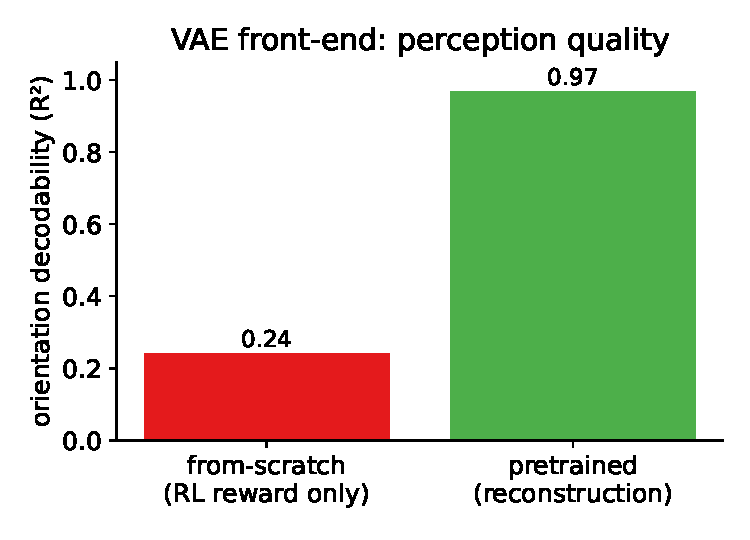
\includegraphics[width=0.52\linewidth]{fig_vae_r2.pdf}
\caption{Orientation decodability ($\Rsq$ of a linear decoder on the front-end's
$\oflat$ features) for the front-end trained from reward versus pretrained on
reconstruction. Reward alone cannot teach orientation perception; reconstruction can.}
\label{fig:vaer2}
\end{figure}

\section{The rescue}
Pretraining the VAE is cheap and decisive. We sample $\sim\!42{,}000$ grayscale
$25\times25$ patches from the environment (blanks, cues, Gabors), train the paper's exact
VAE (convolutional encoder $\to\oflat\to$ latent, transposed-convolution decoder,
reconstruction $+$ small KL) for $\sim\!12$ epochs to a reconstruction loss of $0.0025$,
and freeze the encoder into the front-end. With this single change --- \emph{nothing else
in the network or harness altered} --- the exact paper network \textbf{learns the task on
the first attempt} and climbs above the $0.5$ floor quickly, reaching hit rate $0.79$ with
a false-alarm rate of $0.08$ and a median reaction time of five frames (it presses the
instant it perceives the change).

\section{The VAE is a static, task-parameter-invariant front-end}
A subtle but useful corollary: the VAE is a \emph{per-frame, static} encoder. It
reconstructs one patch at a time and has no notion of motion or time. Task temporal
parameters --- the orientation-noise $\sigma$ and the horizon $T$ --- do not change what the
VAE sees, because the displayed orientations span the full range regardless of $\sigma$.
A single pretrained VAE therefore serves all noise levels and both horizons; there is no
need to re-pretrain per task variant. This both simplifies the pipeline and sharpens the
interpretation of the next chapter: when the long task succeeds without the pretrained VAE,
it is not because the perception problem went away, but because the long horizon admits a
different solution to it.

\section{Why this matters for the architecture choice}
This finding cleanly separates two questions that the earlier history had conflated.
``Does the architecture work?'' and ``Can the front-end see?'' are different. Many of the
collapses catalogued in Chapter~\ref{ch:zoo} on the seven-step task are, in retrospect,
perception failures wearing an architecture's clothes. The methodological upgrade is to
\emph{fix perception first} (frozen pretrained VAE) and only then compare attention/memory
wirings --- which is precisely the controlled setting of Chapters~\ref{ch:deepdive} and
\ref{ch:attention}.

A third perception result (Chapter~\ref{ch:jepa}) qualifies this: perception need not be
solved \emph{before} the architecture if the network carries a self-supervised predictive
auxiliary --- a V-JEPA temporal self-distillation loss --- trained jointly with the policy,
which learns a working front-end from raw pixels or a convolutional encoder with no
pretrained VAE.

\chapter{Finding II --- the horizon decides the strategy}
\label{ch:horizon}

\section{The puzzle}
The history contains a genuine paradox. The cross-talk network reproduced primate cueing
behaviour on the \emph{long} twenty-nine-step task (hit $\approx0.80$) trained from reward
with no pretrained VAE. The \emph{same} architecture, and the exact paper network, collapse
on the \emph{short} seven-step task without a pretrained VAE --- even though the short task
is, by every naive measure, easier (fewer frames, less accumulated noise, a fixed change
time the agent could memorise). How can the easier task be the one that fails?

\section{Two ways to detect a change}
The resolution is that there are two strategies for change detection, and they have
opposite horizon dependence.
\begin{description}
\item[Instantaneous detection.] Compare \emph{this} frame's orientation to the remembered
baseline. This needs accurate per-frame orientation perception, and it detects the change
in a single frame.
\item[Temporal / flow detection.] Notice that \emph{something shifted} in the visual stream
across frames, without representing what the orientation is. The per-frame signal is weak
and noisy, so it must be integrated over many frames to become reliable; it is slow.
\end{description}

\section{The horizon selects between them}
On the long task the change persists for up to $\sim\!18$ frames, so the flow strategy
works: the agent accumulates a weak ``something moved'' signal until it is confident. It
never \emph{needs} accurate perception, and consequently never learns it --- which is
exactly why the long-trained front-end has orientation decodability $\Rsq\approx0.24$ yet
still solves the long task. On the short task the change lasts two frames. There is no time
to integrate, the flow strategy fails, and the only thing that works is instantaneous
perception --- which sparse reward cannot build (Chapter~\ref{ch:perception}). The
pretrained VAE supplies exactly the missing instantaneous perception, and the short task is
solved.

In one sentence: \textbf{the short task removes the temporal-integration escape hatch and
forces abstract, single-frame perception.} Pixel/flow inference is slow; abstract-but-
accurate inference is fast.

\section{The behavioural fingerprint}
The theory makes a sharp, falsifiable prediction that the data already bear out. A model
that detects instantaneously should press the moment the change appears, so its reaction
time should be pinned at change onset and \emph{cannot} be sped up by the cue. The
pretrained-VAE model on the short task does exactly this: median reaction time is five
frames (change onset), essentially flat across change magnitude and across cue validity
(Chapter~\ref{ch:deepdive}). A flow-based model, by contrast, should have long, magnitude-
dependent reaction times. The prediction to complete the argument is a direct comparison of
reaction-time distributions: the from-scratch long-task model should press \emph{late} and
the pretrained-VAE model \emph{early}, the clean signature of ``flow is slow, perception is
fast.''

\section{Consequences for the program}
Two consequences follow. First, \textbf{the short task is the more discriminating test
bed}: because it forecloses the flow shortcut, it forces the network to actually perceive,
and so it exposes architectural differences that the long task hides behind temporal
integration. This is why the cue-attention investigation of Chapter~\ref{ch:attention} is
run on the short task. Second, \textbf{horizon is a design variable, not a nuisance}:
choosing the seven-step task with the frozen VAE gives the cleanest, most mechanism-
revealing setting, while the twenty-nine-step task is the right venue for studying the
\emph{maintenance} of attention across a delay. The empirical paper will want both: the
short task for the sensitivity/criterion story and the long task for the maintenance and
anticipation story.

\chapter{Finding III --- coupling is a precondition for learning}
\label{ch:crosstalk}

A second structural result, established on the long task with the \code{v11} family of
split-pathway networks, is that the coupling between the policy and value streams is not an
optimisation detail --- it is a precondition for the task to be learned at all.

\section{The split-pathway design}
The \code{v11\_part2} network splits the recurrent encoder into two single-head cross-
attention streams that share a deep memory. The \emph{priority} ($\mu$) stream queries the
image and attends over $[\Hone\!\parallel\!\Htwo]$ with an image residual, and its output
$\Zmu$ drives the actor. The \emph{value} ($q$) stream queries the image and attends over
$\Htwo$ with a memory residual, and its output $\Zq$ drives the critic. The cross-talk
lives in the shared deep memory $\Htwo$: the priority stream \emph{writes} it (through
$\Zmu$) and \emph{reads} it back, while the value stream reads the same $\Htwo$. The two
heads are separated but sit on a jointly maintained recurrent register.

\section{The three-way comparison}
Holding the front-end, heads, parameter count, and entire training recipe fixed, three
wirings were trained and evaluated (Table~\ref{tab:crosstalk}):
\begin{enumerate}
\item \textbf{Shared memory (cross-talk).} As above: the two streams coupled through
$\Htwo$, priority driving the actor.
\item \textbf{Independent (no cross-talk).} The same two stream \emph{types}, but each with
its own private memory updated only by its own output --- the minimal edit that removes the
coupling while preserving the split.
\item \textbf{Swapped routing.} Architecturally identical to the coupled model, but the
value stream drives the actor and the priority stream drives the critic.
\end{enumerate}

\begin{table}[t]
\centering
\caption{Coupling between the policy and value pathways is necessary for learning. Same
front-end, heads, parameter count and training recipe; only the inter-pathway wiring
differs. Numbers from the trained checkpoints on the long task.}
\label{tab:crosstalk}
\small
\begin{tabular}{lcccl}
\toprule
Configuration & Accuracy & Hit rate & FA rate & Phenotype \\
\midrule
Shared memory (cross-talk) & \textbf{0.868} & \textbf{0.794} & 0.067 & active, calibrated detector \\
Independent (no cross-talk) & 0.504 & 0.000 & 0.000 & always-wait collapse \\
Swapped routing & 0.420 & 0.000 & 0.000 & always-wait collapse \\
\bottomrule
\end{tabular}
\end{table}

\section{The result}
The coupled model is a genuine psychophysical detector. Both uncoupled controls collapse
completely: across hundreds of episodes they never once declare a change. The independent
model's failure shows that \textbf{a shared substrate is necessary} --- decoupling the
critic's state from the actor's state breaks credit assignment, because the value estimate
that should teach the policy is computed on memory the policy cannot influence. The
swapped-routing failure shows that \textbf{which stream drives the policy also matters} ---
the grounded, image-reading priority stream must command the actor; routing the memory-
grounded value stream to the policy fails even with the coupling intact. The two conditions
are jointly necessary, and the margin --- a fifty-point accuracy gap from a single wiring
edit --- is among the largest the program has produced.

\section{Interpretation and its limits}
The result echoes a deep feature of the biology: in a cortico-basal-ganglia actor--critic,
the actor is updated only through a dopaminergic teaching signal gated by the critic's
reward-prediction error, so severing value from action breaks learning. We are careful,
however, about the mapping. The brain's coupling is a largely scalar, diffusely broadcast
critic-to-actor signal, whereas the model's coupling is a shared recurrent working-memory
register that the actor writes and both read. The model therefore \emph{formalises one
concrete way} to satisfy a constraint the brain satisfies by other means, rather than
replicating the mechanism. The asymmetry result --- that the grounded stream must drive the
policy --- is better motivated by the evidence-accumulation literature (the sensory stage is
the causally necessary one) than by the actor--critic literature, and is the sharpest,
most specific claim the split-pathway work makes.

\section{Standing caveat}
The cross-talk results were obtained on the long task, before the perception finding of
Chapter~\ref{ch:perception}. The split-pathway models read $\mathbf Z$ (the attention
output), not $\mathbf H$ (memory), which on the short task interacts with the perception
and attention findings in ways Chapter~\ref{ch:attention} takes up directly. The coupling
result itself is robust; its expression on the short task with a frozen VAE is one of the
open items in the research plan.

\chapter{The architecture zoo}
\label{ch:zoo}

This chapter catalogues the network variants the program has built and, where trained,
their outcomes. The point is not encyclopaedic completeness but the \emph{pattern} of what
makes attentive behaviour emerge versus collapse. Table~\ref{tab:zoo} is the index;
the prose groups the variants into the families that carry the lessons.

\section{Family A --- memory-as-tokens self-attention (\code{v4}, \code{v5}, \code{v5\_part2})}
The earliest mature line treats the recurrent states as additional tokens. \code{v5} self-
attends over the concatenation $[\,\text{patch}\parallel\Hone\parallel\Htwo\,]$ at every
layer. It works and is highly interpretable: the encoder's first layer becomes a
\emph{top-down, cue-driven spatial orienter} (heads spike to the cued quadrant at cue
onset, follow the cued side, and scale with cue reliability --- the substrate of the
validity effect), while the actor/critic decoder's final layer is a \emph{bottom-up change
detector} that snaps onto the changed quadrant at change onset. This encoder--decoder
dissociation (top-down cue prior vs.\ bottom-up change read-out) is a recurring motif.
\code{v5\_part2} re-architects this as eight-head cross-attention over memory followed by
stacked per-token LSTMs and one-dimensional-convolution heads; it works, and the load-
bearing computation moves into the encoder's memory cross-attention (memory keys are
causally decision-moving, image keys are inert). \code{v4} (a FiLM-encoder sibling) revealed
a cautionary failure mode: a FiLM gain that initialises to zero with no ``$+1$'' offset
makes the attention a structurally uniform global average-pool --- the first appearance of
the ``identity floor matters'' lesson that returns in Chapter~\ref{ch:attention}.

\section{Family B --- bottleneck residuals (\code{v8}, \code{v8\_part2}, \code{v9})}
This line tightens how visual information reaches memory. \code{v8} routes the attention
residual through the previous memory rather than the image, so visual content can only
flow through attended values; it works, with very fast reaction times and an emergent
dedicated patch-reading head. Push the bottleneck further --- memory-only keys and values
(\code{v8\_part2}) or queries drawn from memory rather than the image (\code{v9}) --- and the
models collapse to always-wait. The diagnosis is consistent: removing the grounded image
fallback puts perception on a knife-edge, so the policy retreats to the safe action. This
is the same lesson the split stream of \code{v11} was designed to fix.

\section{Family C --- split priority/value pathways (\code{v11}, \code{v11\_part2--5})}
The split-pathway family is the program's most productive line and the subject of
Chapter~\ref{ch:crosstalk}. \code{v11} (parallel streams, heads read both transformer
outputs) fixed the always-wait collapse by grounding the priority stream in the image.
\code{v11\_part2} added the deep memory to the priority keys and split the readout (priority
$\to$ actor, value $\to$ critic); it is the canonical working cross-talk model, and its
headline is the \emph{reliability-scaled} cueing benefit that the un-split \code{v11}
lacked. \code{v11\_part3} (swapped readout) and \code{v11\_part4} (independent, no cross-
talk) both collapse to chance --- the necessity results of Table~\ref{tab:crosstalk}.
\code{v11\_part5} ports the working cross-talk model to the distractor task and yields a
clean double dissociation: biasing the priority stream swings the decision while leaving
value flat, biasing the value stream moves value but never the decision; the distractor is
filtered in the \emph{decision} pathway (decodable from sensory memory but cold to the
priority map --- ``seen but not acted upon''), and value gates \emph{whether} the priority
filter is deployed in a binary, engage/abandon fashion.

\section{Family D --- codebook / vector-quantised attention (\code{v12}, \code{v12\_part2/3})}
Motivated by an ``attention as a lookup table / superior-colliculus microstimulation''
analogy, this line makes the attention values a learnable codebook. The hard sampled/STE
version failed to learn (a gradient mismatch under prioritised replay re-encoding); the
soft-attention codebook (\code{v12}) is differentiable and trains. The adaptive-codebook
extensions add a deformation with an energetic maintenance cost (\code{v12\_part2}) and an
EMA codebook written by a gated image-content stream (\code{v12\_part3}); the EMA-only
variant collapses (a catch-22 in which the magnitude penalty drives the very signal the EMA
should consolidate to zero), which is what motivated the gradient-learned-codebook fix.

\section{Family E --- predictive-coding and energy modulation (\code{v13}, \code{v14}, \code{v15})}
The most exploratory line asks whether a self-supervised recurrent dynamical system can be
repurposed for the task by ``energy modulation'' rather than retraining. \code{v13} freezes
a JEPA-style predictive-coding encoder and adds an energy stream that modulates its
dynamics, training only the energy and heads. \code{v14} runs two gradient-firewalled
modules concurrently --- a self-supervised module (JEPA latent, no pixels) and a
reinforcement-learning module --- that share state forward but never gradients. \code{v15}
adds a VQ-VAE-style energy term on top of a gradient-learned codebook that provably reduces
to the working codebook when the energy is off. These are mechanism studies more than
performance plays; on the current low-bandwidth task they are expected to track their
working bases, with the energy/adaptation machinery reserved for higher-bandwidth tests.

\begin{table}[t]
\centering
\caption{Index of the architecture zoo. ``Outcome'' is the trained behaviour where a run
exists; many variants are mechanism studies built and unit-tested but reserved for a
higher-bandwidth task. \checkmark\ = learns/works, $\times$ = collapses, $\circ$ = built,
not yet a decisive run.}
\label{tab:zoo}
\scriptsize
\begin{longtable}{p{2.3cm}p{6.8cm}p{2.0cm}}
\toprule
Variant & Mechanism (what is varied) & Outcome \\
\midrule
\endhead
\code{v5} & memory-as-tokens self-attention, $[\text{patch}\parallel\Hone\parallel\Htwo]$ & \checkmark\ (cue-orienting) \\
\code{v5\_part2} & 8-head cross-attn over memory $\to$ stacked LSTMs $\to$ conv heads & \checkmark\ \\
\code{v4} & FiLM-encoder sibling; revealed zero-init gain $\Rightarrow$ uniform attn & $\circ$ (diagnostic) \\
\code{v7} & \code{v5\_part2} arch on cued-side distractor task & $\circ$ \\
\code{v8} & H1-residual bottleneck (visual info only via attended values) & \checkmark\ (fast RT) \\
\code{v8\_part2} & memory-only K/V (patch = queries only) & $\times$ (always-wait) \\
\code{v8\_part3} & predictive-comparator write gate (surprise opens LSTM2 input) & $\circ$ \\
\code{v9} & memory-query attention (queries from $\Hone$, not image) & $\times$ (collapse) \\
\code{v11} & parallel priority $\parallel$ value streams; heads read both $\mathbf Z$ & \checkmark\ (hit 0.63) \\
\code{v11\_part2} & $+$\,deep memory in priority keys, split readout (the cross-talk) & \checkmark\ (hit 0.80) \\
\code{v11\_part3} & \code{v11\_part2} with actor/critic readout swapped & $\times$ (chance) \\
\code{v11\_part4} & independent streams, no shared memory & $\times$ (chance) \\
\code{v11\_part5} & cross-talk on the distractor task & \checkmark\ (double dissoc.) \\
\code{v12} & soft codebook attention, static learnable codebook & \checkmark\ (soft) \\
\code{v12\_part2} & adaptive codebook deformation $+$ energetic cost & $\circ$ \\
\code{v12\_part3} & EMA codebook written by a gated content stream & $\times$ (EMA-only) / $\circ$ (gated) \\
\code{v13} & frozen predictive-coding encoder $+$ energy-modulation stream & $\circ$ \\
\code{v14} & two gradient-firewalled modules (self-supervised $\perp$ RL) & $\circ$ \\
\code{v15} & gradient codebook $+$ VQ-VAE energy (reduces to \code{v12}) & $\circ$ \\
\code{setsize9} & cross-talk arch on the 9-stimulus set-size task & $\circ$ \\
\bottomrule
\end{longtable}
\end{table}

\section{What the zoo says in aggregate}
Three regularities cut across the families. (1) \textbf{A grounded image pathway is
required}: every variant that removes the bottom-up route to either memory or the decision
collapses to always-wait. (2) \textbf{Routing, not representation, decides the phenotype}:
identical encoders produce a working detector or a chance model depending only on which
stream drives the policy and whether a shared substrate couples value to action. (3)
\textbf{Interpretability is an emergent property of the right wiring}: the variants that
learn also expose clean, manipulable attention maps (cue-orienting encoders, change-locked
decoders), whereas the collapsed variants expose nothing. These regularities are the
empirical backbone of the recommendation in Chapter~\ref{ch:recommendation}.

\chapter{Finding IV --- the working model reproduces the paper}
\label{ch:deepdive}

With perception fixed by the frozen VAE (Chapter~\ref{ch:perception}), the exact paper
network on the seven-step task is a real psychophysical detector, and it reproduces the
core behavioural figures of the published manuscript. This chapter is the quantitative
deep dive on that model.

\section{Baseline behaviour}
Under a greedy policy the model catches $79\%$ of real changes, false-alarms on $8\%$ of
no-change trials, and presses with a median reaction time of five frames --- the instant a
change can appear. It is not a degenerate $0.5$ model; it discriminates change from
no-change with a healthy sensitivity.

\section{Psychometrics: the reliability-scaled cueing benefit}
The discriminating test of attention is not accuracy but the \emph{cueing signature}: a
detection advantage for changes at the cued location that scales with how reliable the cue
is. We measured it by presenting a cue of a given validity, forcing the change at the cued
($S_1$) or uncued ($S_4$) location at a fixed magnitude $\Delta$, and fitting a
four-parameter logistic to the detection-rate-versus-$\Delta$ curve. The threshold (the
logistic's position) is the sensitivity readout. The result (Fig.~\ref{fig:psy},
Table~\ref{tab:thr}) is the paper's headline:
the cued threshold falls below the uncued threshold by an amount that \emph{grows
monotonically with validity} --- a negligible $+1.5^\circ$ at $25\%$, a robust $+7.5^\circ$
at $100\%$. At $25\%$ validity (no predictive spatial information) there is essentially no
cueing effect; at $100\%$ there is a large one, carried by the threshold/sensitivity
parameter rather than the guess or lapse rates. This is the canonical sensitivity-enhancing
signature of primate spatial attention, reproduced.

\begin{table}[t]
\centering
\caption{Psychometric thresholds (four-parameter logistic position, degrees) for cued
versus uncued changes by cue validity, and the resulting cueing benefit. The benefit scales
with validity --- the paper's central behavioural result.}
\label{tab:thr}
\small
\begin{tabular}{lccc}
\toprule
Cue validity & Cued threshold & Uncued threshold & Cueing benefit \\
\midrule
25\% & 13.6 & 15.1 & $+1.5$ \\
50\% & 14.3 & 19.2 & $+4.8$ \\
75\% & 11.3 & 17.5 & $+6.1$ \\
100\% & 11.8 & 19.4 & $\mathbf{+7.5}$ \\
\bottomrule
\end{tabular}
\end{table}

\begin{figure}[t]
\centering
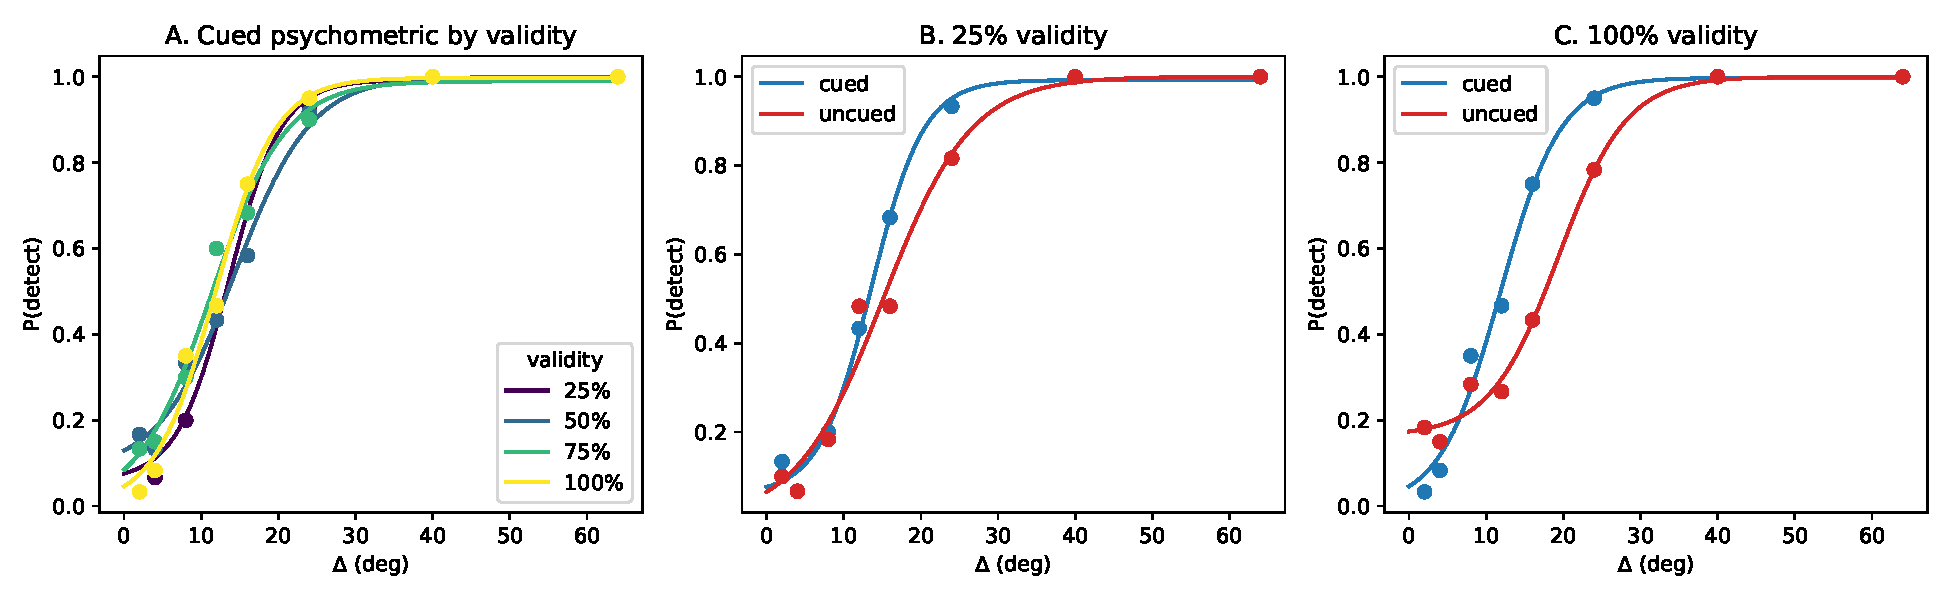
\includegraphics[width=0.49\linewidth]{fig_psychometric.pdf}\hfill
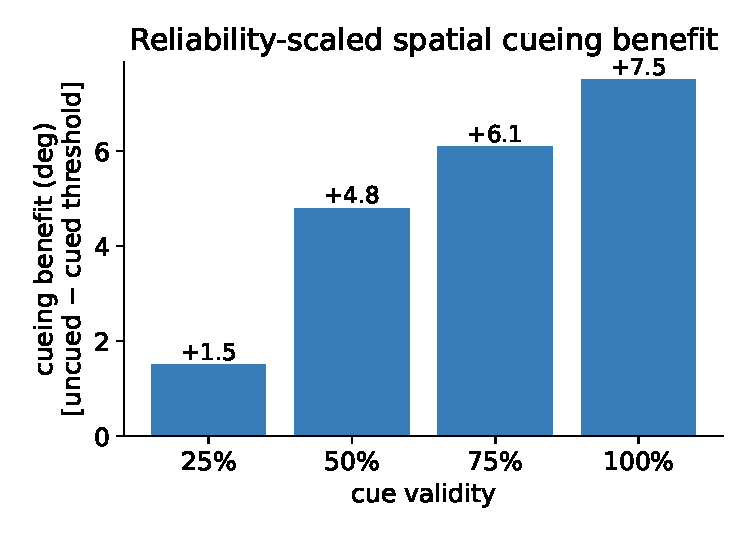
\includegraphics[width=0.46\linewidth]{fig_cueing_benefit.pdf}
\caption{Left: psychometric detection-rate curves by cue validity (cued changes) and the
cued-versus-uncued comparison at low and high validity. Right: the cueing benefit
(uncued$-$cued threshold) scales monotonically with validity.}
\label{fig:psy}
\end{figure}

\section{Chronometrics: the reaction-time story}
Reaction time is pinned at change onset ($\approx5$ frames) with only a faint difficulty
effect (slightly slower for the hardest changes) and \emph{no} reaction-time cueing benefit
(cued and uncued reaction times are equal to within $0.06$ frames; Fig.~\ref{fig:chrono}).
This is not a failure to reproduce so much as a consequence of the instantaneous-perception
mechanism (Chapter~\ref{ch:horizon}): the cue moves the decision \emph{criterion}
(accuracy) but cannot speed a response that is already at the floor. It is a specific,
testable prediction --- good perception yields a criterion-shift cueing effect without a
reaction-time benefit --- and it is one of the places the model diverges, informatively,
from a slower flow-based detector.

\begin{figure}[t]
\centering
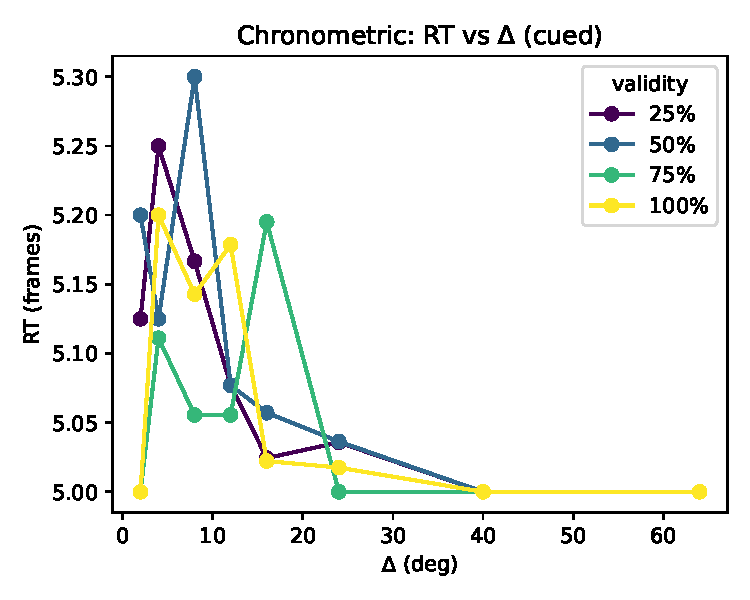
\includegraphics[width=0.46\linewidth]{fig_chronometric.pdf}\hfill

\includegraphics[width=0.49\linewidth]{fig_causal.pdf}
\caption{Left: reaction time versus change magnitude by cue validity --- pinned near five
frames, a weak difficulty effect, no validity benefit. Right: the causal attention
manipulation --- biasing attention toward the changed location improves detection,
biasing it toward a distractor impairs it, without inducing false alarms.}
\label{fig:chrono}
\end{figure}

\section{Causal attention manipulation}
The paper's causal result is that attention is causally linked to perceptual sensitivity,
not merely correlated with it. We tested this by clamping the attention onto a target
patch during the stimulus frames and measuring detection of a sub-threshold change
(Fig.~\ref{fig:chrono}, right). Biasing attention \emph{toward} the changed location
improves the hit rate from $0.265$ to $0.350$ ($+8.5\%$); biasing it \emph{toward a
distractor} impairs it to $0.185$ ($-8.0\%$); and biasing attention on a no-change trial
barely moves the false-alarm rate ($+1\%$). The effect is bidirectional and clean ---
exactly the hallmark causal signature of attention (enhanced sensitivity at the attended
location, like sub-threshold superior-colliculus or frontal-eye-field microstimulation).
Crucially, biasing attention does not \emph{manufacture} a change percept; it gates
\emph{which} location's content reaches the decision.

\section{Scorecard}
On the seven-step task the working model reproduces the two results the published
manuscript is built on --- the reliability-scaled psychometric cueing benefit and the
causal attention-to-sensitivity link --- cleanly. The reaction-time cueing benefit does not
reproduce (reaction time is floored by instantaneous detection), and the attention-
\emph{dynamics} story is its own subject, taken up next.

\chapter{Finding V --- attention versus memory, and the cue-attention question}
\label{ch:attention}

The deep dive raised a mechanistic question that is, at the time of writing, the program's
live frontier: in the canonical multiplicatively-gated model, the cueing \emph{behaviour}
is real and graded, yet the per-frame attention map does not orient to the cue. This
chapter sets out the dissociation, the mechanism behind it, and the matched family of
architectures we are training to resolve it.

\section{The cue modulates behaviour}
First, to be unambiguous: the cue strongly modulates the model's behaviour. The detection
threshold for a cued change is up to $7.5^\circ$ lower than for an uncued change, and the
benefit scales with validity (Chapter~\ref{ch:deepdive}). The model reads the cue, holds
it, and uses it. The question is not \emph{whether} the cue is used but \emph{through what
internal variable}.

\section{The attention is change-locked, not cue-locked}
We measured the four-patch attention map at every frame for a $100\%$ cue at $S_1$ with a
$25^\circ$ change at $S_1$ (Fig.~\ref{fig:attn_change}). The attention is uniform
($\approx0.25$ per patch) through the cue frame and the entire delay, and it sharpens onto
$S_1$ only at frame $5$ --- the moment the change appears. The full $4\times4$ query-key
matrix at the cue frame is essentially uniform, so this is not an artefact of how the map
is summarised: there is no cue-driven structure to summarise. A no-change control confirms
the reading (Fig.~\ref{fig:attn_nochange}): with the same $100\%$ cue but no change, the
attention stays flat across all seven frames (maximum deviation from uniform $0.039$). The
attention fires at a location when, and only when, that location \emph{changes}.

\begin{figure}[t]
\centering
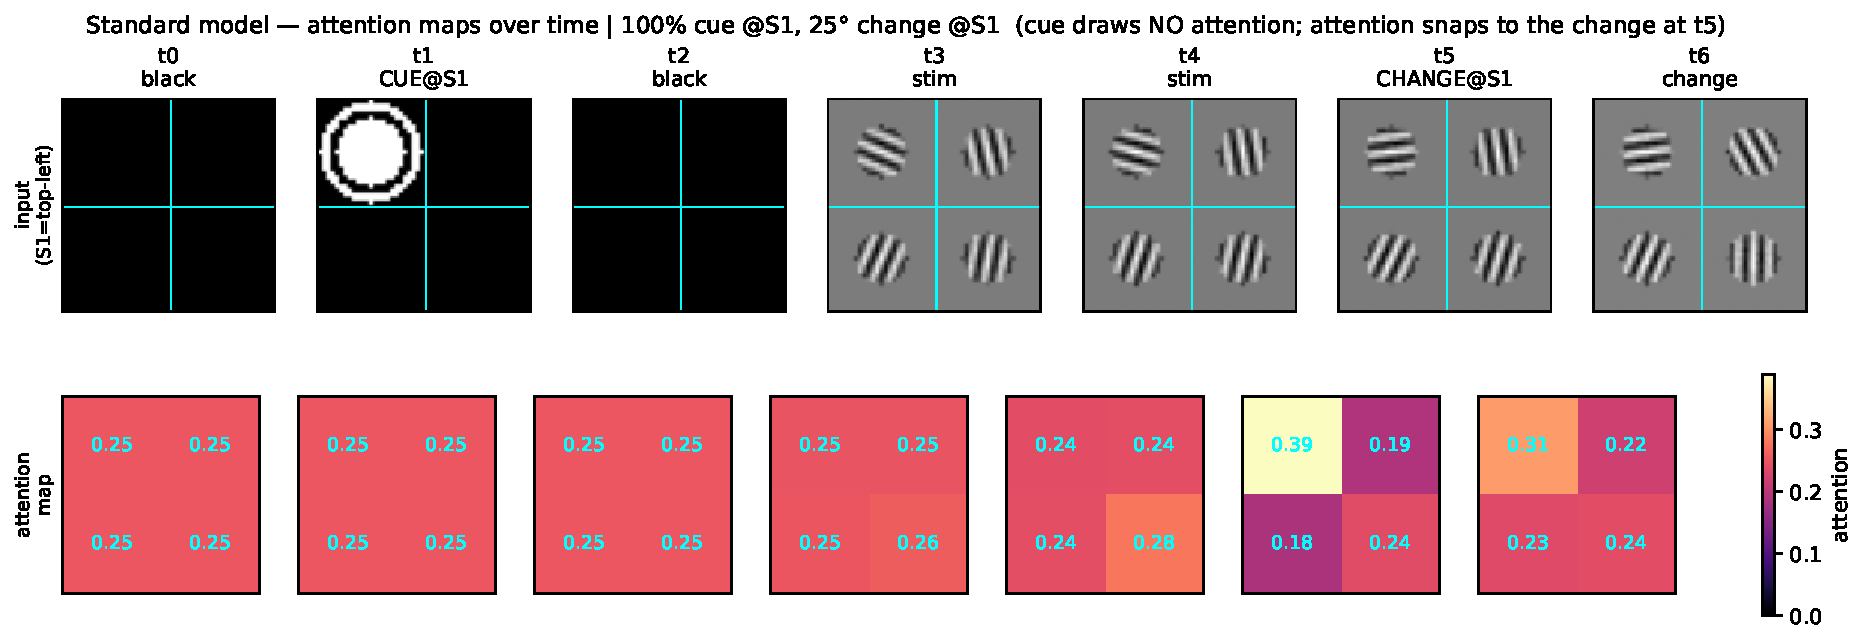
\includegraphics[width=0.95\linewidth]{fig_attention_maps_S1.pdf}
\caption{Per-frame attention (top: input frames; bottom: $2\times2$ attention map, S1 =
top-left) for a $100\%$ cue at $S_1$ with a $25^\circ$ change at $S_1$. The cue (frame 1)
draws no attention; the attention concentrates on $S_1$ only at the change (frame 5).}
\label{fig:attn_change}
\end{figure}

\begin{figure}[t]
\centering
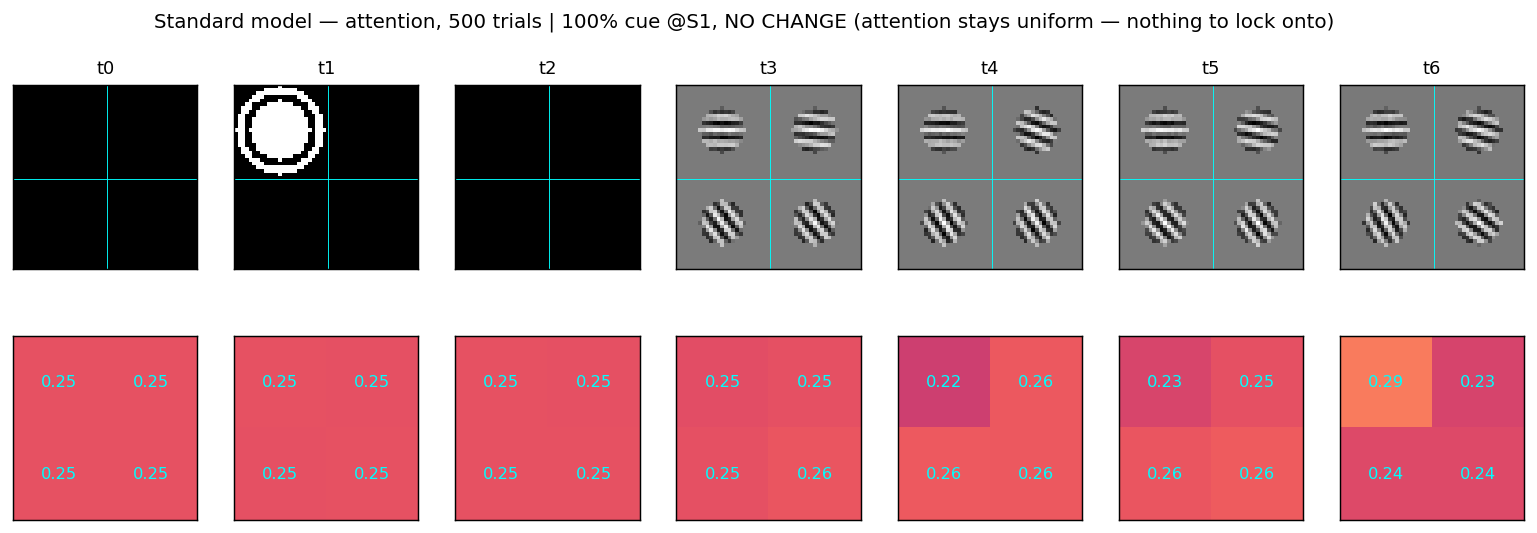
\includegraphics[width=0.85\linewidth]{fig_attention_maps_S1_nochange.png}
\caption{No-change control, $500$ trials, $100\%$ cue at $S_1$. With nothing to lock onto
the attention stays uniform across every frame --- the cue alone never moves it.}
\label{fig:attn_nochange}
\end{figure}

\section{Where the cue actually lives}
If not in the attention, where? In the recurrent memory. Decoding from the flattened memory
$\mathbf H$ at the pre-change frame, both the cued \emph{location} ($S_1$ vs.\ $S_4$) and
the \emph{validity} ($25/50/75/100\%$) are recovered at $100\%$ accuracy (chance $50\%$ and
$25\%$). The cue and its reliability are perfectly maintained in working memory, where they
set the decision threshold; the attention, meanwhile, is a bottom-up change detector. This
is a clean dissociation: \textbf{cue $\to$ behaviour: yes; cue $\to$ attention map: no}.

\section{The mechanism}
The dissociation has a transparent cause in the multiplicative form
(Eq.~\ref{eq:mult}). Because $\mathbf Q=(\X\mathbf W_{XQ})\odot(\Hone\mathbf W_{HQ})$, the
query magnitude is gated by the memory projection. At the cue frame the memory has not yet
built up, the gate $\lvert\Hone\mathbf W_{HQ}\rvert$ is near zero ($\approx0.02$), and the
queries and keys collapse toward zero, so the attention is uniform. The model is then
\emph{free} to keep that gate small, because the cue reaches memory through the image
residual $\X$ in $\mathbf Z=\X+\mathbf V_{\text{filt}}$ and the LSTM, without the attention
ever needing to orient. The multiplicative form, in short, \emph{admits} a memory-only
solution, and on the seven-step task with a frozen VAE and a memory readout, the harness
finds it.

\section{The open question}
This is where honesty is required. The lab's other models --- multi-head, cross-attention
variants in the spirit of \code{v5} and \code{v11} --- reliably \emph{do} orient attention
to the cue, across many trained networks. So orienting is clearly achievable with these
mechanisms; the multiplicative-gated reproduction is the outlier. The cause is therefore
\emph{some feature of our specific reproduction} --- the gate form, the head count, the
memory readout, the harness, the frozen front-end --- not a property of memory-gated
attention in general. We do not yet know which feature, and we are not guessing: we are
testing it directly with a matched family of architectures.

\section{The matched family under test}
Each variant changes exactly one thing about the attention/memory wiring on the identical
base (frozen VAE, harness, readout dimension), so any difference in whether attention
orients to the cue is attributable to that change. Table~\ref{tab:family} lists them.

\begin{table}[t]
\centering
\caption{The matched family of attention/memory wirings under training to resolve the
cue-attention question. All share the frozen-VAE front-end, the PAC$+$QR-DQN$+$PER harness,
and the $4096$-d readout.}
\label{tab:family}
\small
\begin{tabular}{p{2.2cm}p{7.2cm}p{2.0cm}}
\toprule
Variant & What it changes about the feedback / memory & Status \\
\midrule
multiplicative & canonical $\mathbf Q=(\X\mathbf W)\odot(\Hone\mathbf W)$ (the reproduction) & works; change-locked \\
affine & memory derives a scale-\emph{matrix} $+$ shift: $\X'=\Gamma(\Hone)\X+\beta(\Hone)$ & \textbf{failed (always-wait)} \\
dualhead & a memory-free sensory head $\parallel$ the multiplicative feedback head & works; weak orient \\
two-lstm & split memory: $\Hone$ feeds attention, $\Htwo$($\Hone$) feeds heads & \textbf{best detector} \\
crossattn & additive cross-talk: $\mathbf K,\mathbf V=[\X\parallel\Hone]$, two LSTMs from $\mathbf Z$ & works; memory-routed \\
dualmem & memories \emph{query}: $\mathbf Q([\Hone\parallel\Htwo])$, $\mathbf K,\mathbf V=[\X\parallel\Hone\parallel\Htwo]$ & works; memory-routed \\
\bottomrule
\end{tabular}
\end{table}

\section{Results: the family resolves the question}
All six variants are now trained to $\sim$$18{,}750$ iterations on the identical frozen-VAE
base, and each was evaluated greedily for behaviour ($250$ episodes on \code{validity4}) and
for cue-orienting with the same $100\%$-cue protocol used above: a fully reliable cue, the
attention to the \emph{cued} patch recorded across all seven frames, in a no-change
condition (so any pre-change bias toward the cued location is cue-driven, not change-driven)
and a change condition (so the change-locked component is visible). The
\emph{cue-orienting index} is the cued-patch attention at the pre-change stimulus frames
($t_{3,4}$) minus uniform; the \emph{change-locked spike} is the cued-patch attention jump
at the change frame ($t_5$). Table~\ref{tab:familyresults} reports both alongside behaviour;
Figures~\ref{fig:varattn} and~\ref{fig:varbeh} plot them.

\begin{table}[t]
\centering
\caption{Matched-family results. Behaviour is greedy on \code{validity4} ($T=7$);
cue-orient $>0$ means the attention is biased toward the cued location \emph{before} the
change (cue-driven). The headline: no variant produces a large positive cue-orient, while
two of them (\code{crossattn}, \code{dualmem}) attend markedly \emph{away} from the cued
image patch --- the cueing effect is carried by memory across the whole family.}
\label{tab:familyresults}
\small
\begin{tabular}{lccccrr}
\toprule
Variant & correct & hit & FA & median RT & cue-orient & chg-spike \\
\midrule
multiplicative & $0.804$ & $0.705$ & $0.091$ & $5.0$ & $-0.011$ & $+0.143$ \\
affine         & $0.504$ & $0.000$ & $0.000$ & ---   & $+0.014$ & $-0.001$ \\
dualhead       & $0.820$ & $0.708$ & $0.088$ & $5.0$ & $+0.038$ & $-0.002$ \\
two-lstm       & $\mathbf{0.872}$ & $\mathbf{0.836}$ & $0.094$ & $5.0$ & $+0.008$ & $+0.216$ \\
crossattn      & $0.840$ & $0.760$ & $0.080$ & $5.0$ & $-0.179$ & $-0.011$ \\
dualmem        & $0.828$ & $0.750$ & $0.079$ & $5.0$ & $-0.174$ & $+0.002$ \\
\bottomrule
\end{tabular}
\end{table}

\begin{figure}[t]
\centering
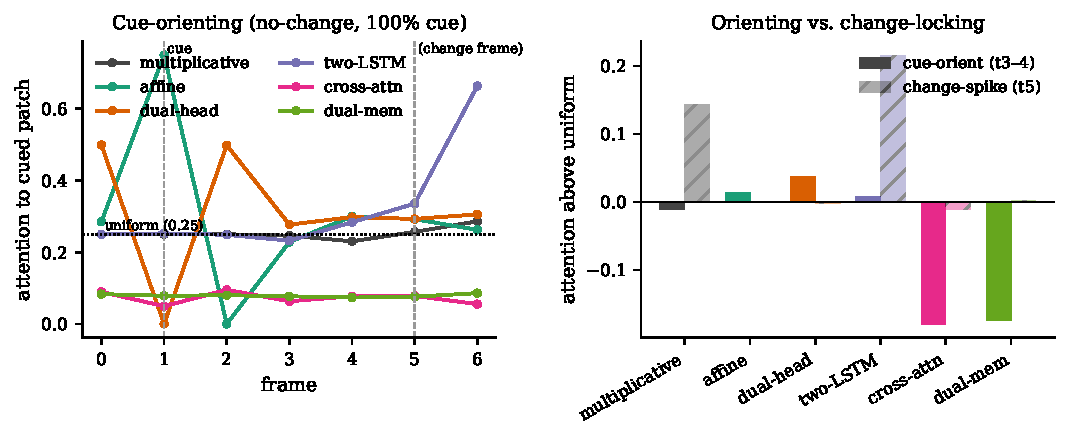
\includegraphics[width=0.99\linewidth]{fig_variants_attention.pdf}
\caption{\emph{Left:} attention to the cued patch across the seven frames, no-change,
$100\%$ cue, for every working variant. All hover near or below uniform ($0.25$) through the
cue and delay; none lifts the cued location before the change. \emph{Right:} the
cue-orienting index ($t_{3,4}$, solid) and the change-locked spike ($t_5$, hatched). The
models that read a direct image$\to$attention path (\code{multiplicative}, \code{two-lstm})
show a clear change-lock and no orienting; \code{crossattn} and \code{dualmem} sit well
below uniform on the cued image patch --- they route the cued location through memory rather
than attending it.}
\label{fig:varattn}
\end{figure}

\begin{figure}[t]
\centering
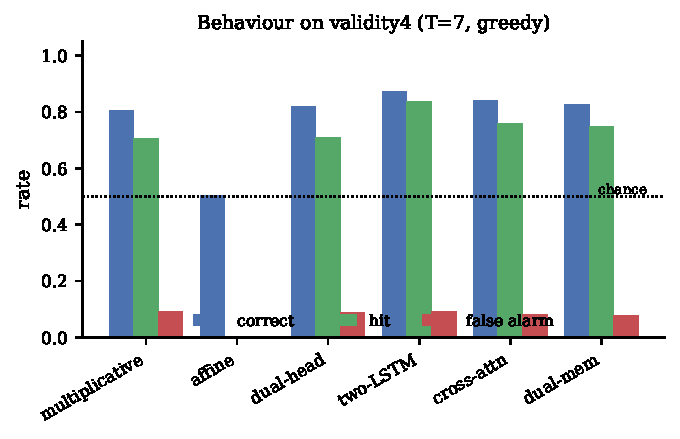
\includegraphics[width=0.62\linewidth]{fig_variants_behavior.pdf}
\caption{Behaviour on \code{validity4}. Five of six variants learn the task; \code{affine}
collapses to always-wait (hit $=0$, no false alarms, $P(\text{press})\le0.004$ even on a
clear $60^\circ$ change). \code{two-lstm} is the best detector.}
\label{fig:varbeh}
\end{figure}

The matched family answers the question, and not in the direction the single early data
point suggested. \textbf{No variant restores strong cue-orienting attention on this task.}
The largest positive cue-orienting index is \code{dualhead}'s sensory head at $+0.038$ ---
real but small, and too weak to carry an attention-allocation figure. The
\code{multiplicative} and \code{two-lstm} models are change-locked exactly as the deep dive
described (spike $+0.143$, $+0.216$; orient $\approx0$). And the two richest cross-talk
wirings, \code{crossattn} and \code{dualmem}, attend \emph{below} uniform at the cued image
location ($-0.179$, $-0.174$): given the choice between image keys and memory keys, they
spend their attention on memory, leaving the bottom-up image patch under-weighted. The
dissociation of Chapter~\ref{ch:attention} is therefore not a quirk of the multiplicative
gate; it is \emph{general} across six attention/memory wirings on this perception front-end
and this task. Reward, on the seven-step task, does not make attention orient to the cue ---
it makes \emph{memory} hold the cue.

\paragraph{A correction.} An earlier reading of a single partially-trained \code{affine}
checkpoint suggested it ``already attends the cue.'' That was premature: fully evaluated,
\code{affine} never presses (Fig.~\ref{fig:varbeh}), so its attention is not behaviourally
meaningful, and the apparent cue structure does not survive into a model that performs the
task. The lesson --- verify behaviour before reading an attention map --- is the same one
the dissociation itself teaches.

\section{Why this matters}
For the empirical manuscript, the behavioural reproduction (Chapter~\ref{ch:deepdive})
stands regardless. But the result reshapes the attention-map story in two useful ways.
First, it converts the open question into a \emph{finding}: across this family, the cueing
effect is memory-borne, and the attention map is a bottom-up change detector --- a
defensible, falsifiable claim now backed by six wirings rather than one. Second, it picks
the network: \code{two-lstm} is both the best detector and a minimal, paper-faithful change
to the published multiplicative attention (a second stacked memory), so it is the natural
network to carry forward, with the memory-driven account of cueing stated plainly rather
than hidden behind an attention figure that the mechanism does not support. If a future
task with a longer delay or a harder cue \emph{forces} pre-orienting, this same family is
the instrument to re-run; on the seven-step task, the honest figure is the change-locked
one.

\chapter{Finding VI --- perception can be learned without a pretrained VAE: V-JEPA self-distillation}
\label{ch:jepa}

Chapters~\ref{ch:perception} and \ref{ch:recommendation} establish two facts that
together harden into a recommendation: on the short seven-step task perception cannot be
learned from reward (a from-scratch VAE collapses to always-press, orientation
$\Rsq=0.24$ against the pretrained VAE's $0.97$), and the cure is a \emph{frozen
pretrained VAE} front-end, declared one of two non-negotiables. This chapter is a third
perception result that qualifies that recommendation rather than overturning it. It shows
perception \emph{can} be learned jointly with reinforcement learning, with no pretrained or
frozen VAE, when the network is given a self-supervised auxiliary: a V-JEPA temporal
self-distillation loss (prototype-softmax, DINO/iBOT-style, EMA teacher, student$@t$
predicting teacher$@t{+}1$) trained jointly with the actor--critic. Paired with either time
to integrate (frame-repeat from raw pixels, $\sim0.90$ training rolling correct) or a
capable convolutional front-end (an SE-ResNet, $\sim0.87$ greedy correct with a sharp,
fully dissected covert-cueing algorithm), the auxiliary turns the perception bottleneck
into a solvable joint problem. The chapter also reports informative negatives that fence the
recipe: externalising a categorical softmax simplex as the working memory kills task
learning; a plain SmoothL1 latent-regression JEPA undergoes representational collapse; and
the matrix-affine two-LSTM feedback wiring collapses to chance under either the JEPA or a
VAE, isolating the fault to the wiring. The cross-cutting lesson is that the perceptual
front-end, not memory size, sets the attention strategy: a strong per-frame encoder yields a
sharp attention-driven solution, while learning from held pixels yields a diffuse,
recurrence-driven one. Because predicting future latents is arguably more biologically
plausible than supervised reconstruction-pretraining, this route is also the more neurally
defensible way to obtain a working front-end.

\section{The question Chapter 5 left open}
Chapter~\ref{ch:perception} draws a clean line between two questions that the earlier
architecture history had conflated: \emph{can the front-end see?} and \emph{does the
architecture work?} On the seven-step task the answer to the first was decisively negative
when perception was asked to emerge from reward alone. A VAE front-end trained end-to-end
from the reinforcement signal collapses to the \emph{always-press-at-the-deadline}
degenerate policy --- hit rate $1.000$, false-alarm rate $1.000$ on no-change trials,
overall accuracy $0.515$, reaction time pinned at frame $5$ --- and a linear probe confirms
the cause: orientation is decodable from the from-scratch encoder at only $\Rsq=0.24$ versus
$\Rsq=0.97$ for the pretrained VAE. Freezing a pretrained VAE rescues learning on the first
attempt (hit $0.79$, false-alarm $0.08$). Chapter~\ref{ch:recommendation} then elevates the
frozen pretrained VAE to one of \emph{two non-negotiables}.

That recommendation is correct \emph{as a statement about supervised reconstruction-
pretraining applied to a static, per-frame encoder}. It leaves a sharper question open: is
the pretrained VAE necessary because perception is genuinely unlearnable jointly with the
policy, or because reconstruction from reward is simply the wrong learning signal? This
chapter answers that perception is learnable jointly with the policy --- provided the
network carries a \emph{self-supervised predictive} auxiliary that does not depend on the
reward, and provided it is paired with one of two enablers that give the recurrence enough
perceptual purchase to use it. The result qualifies the non-negotiable: a frozen pretrained
VAE is one way to satisfy the perception requirement, not the only way.

\section{The auxiliary: V-JEPA temporal self-distillation}
The auxiliary is a video-JEPA self-distillation loss attached to the recurrent cell and
trained jointly with the actor--critic. A projection head reads the continuous xLSTM cell
output and emits, for each of $4$ heads, a softmax over $256$ prototypes. A teacher network
is an exponential moving average of the student (decay $0.996$); its outputs are centred
(centre momentum $0.9$) and sharpened (student temperature $0.1$; teacher temperature
warming from $0.04$ to $0.07$ over a $300$-iteration warm-up). The student's prototype
distribution at time $t$ is trained to predict the teacher's distribution at time $t{+}1$
--- a temporal, predict-the-next-latent target rather than a masked-spatial one. The loss
enters total optimisation only through a coefficient (\texttt{jepa-coef} $0.5$); crucially
it \emph{does not change the memory}, which stays a continuous xLSTM and is never itself
softmaxed. The prototype-softmax with centring and sharpening supplies the anti-collapse
machinery that, as Section~\ref{sec:jepa-negatives} shows, a naive latent loss lacks.

The diagnostic for whether the auxiliary is doing real work is the trajectory of the JEPA
loss. A loss that stays flat means the auxiliary never engages; a loss that drops to
$\approx0$ means representational collapse to a constant; a loss that descends to a healthy
non-zero plateau means structured, non-degenerate predictive learning. On the
frozen-colour-VAE control --- the exact paper network with the auxiliary bolted on --- the
auxiliary is a pure add-on and is not load-bearing: both feedback wirings reach $\sim0.85$
training rolling correct (peak $\sim0.90$) whether or not the JEPA engages, and \emph{whether
it engages at all is set by the feedback wiring}. Under cross-attention feedback the loss
falls $\sim3.7\times$ (first-200 mean $5.35\to$ late-200 mean $1.24$); under FiLM feedback it
sits inert ($5.32\to4.99$) --- though this FiLM run stopped early at $16{,}385$ of a
configured $50{,}000$ iterations, so its inertness is partly confounded with training length.
With perception already solved by the frozen VAE, the auxiliary neither helps nor hurts. Its
value appears only where there is no frozen VAE to solve perception for it.

Table~\ref{tab:jepa} summarises every variant studied in this chapter; the two routes that
make pixel-level learning work (Sections~\ref{sec:jepa-resultA} and \ref{sec:jepa-resultB})
and the three negatives that fence the recipe (Section~\ref{sec:jepa-negatives}) are
developed below.

\begin{table}[t]
\centering
\small
\begin{tabular}{@{}lllllrrll@{}}
\toprule
Model & Front-end & Feedback & JEPA flavour & Env & $d_{\text{mem}}$ & Iters & Rolling correct & Status \\
\midrule
paper\_jepa\_vae & frozen colour VAE & FiLM & proto-softmax & vda4 T7 & 1024 & 16385 & 0.846 (peak 0.90) & works (JEPA inert) \\
paper\_jepa\_vae & frozen colour VAE & crossattn1 & proto-softmax & vda4 T7 & 1024 & 49999 & 0.863 (peak 0.90) & works (JEPA engaged) \\
paper\_jepa\_fr\_novae & pixel (no VAE) & crossattn1 & proto-softmax & vda4 FR$\times$5 & 1024 & 33674 & 0.862 (final 0.895) & works \\
paper\_jepa\_fr\_novae & pixel (no VAE) & crossattn1 & proto-softmax & vda4 FR$\times$5 & 512 & 21240 & 0.807 (final 0.765) & works \\
paper\_jepa\_fr\_novae & pixel (no VAE) & crossattn1 & proto-softmax & vda4 FR$\times$5 & 256 & 15981 & 0.828 (final 0.848) & works \\
paper\_jepa\_fr\_novae & pixel (no VAE) & crossattn1 & proto-softmax & vda4 FR$\times$5 & 128 & 15327 & 0.828 (final 0.820) & works \\
paper\_jepa\_conv & SE-ResNet conv & crossattn1 & proto-softmax & vda4 T7 & 128 & 12989 & 0.870 (greedy 0.865) & works \\
paper\_jepa\_conv & SE-ResNet conv & affine\_ew & proto-softmax & vda4 T7 & 128 & 6662 & 0.867 (greedy $\sim$0.83) & works \\
paper\_jepa\_grid9 & SE-ResNet conv & crossattn1 & proto-softmax & vda9 3$\times$3 & 128 & $\sim$361 & 0.65 (final 0.695) & mid-training \\
paper\_jepa\_grid9 & SE-ResNet conv & affine\_ew & proto-softmax & vda9 3$\times$3 & 128 & $\sim$353 & 0.74 (final 0.803) & mid-training \\
paper\_jepa\_smem & pixel (no VAE) & crossattn1 & softmax-as-memory & vda4 FR$\times$5 & 1024 & 4211 & 0.003 (collapse) & failed \\
affine2lstm\_jepa & conv 4$\times$4, no VAE & matrix-affine & SmoothL1 latent & vda T7 & H2 cell & 18749 & 0.498 (chance) & collapsed \\
paper\_affine2lstm\_vae & conv 4$\times$4, VAE & matrix-affine & none (VAE ctrl) & vda T7 & H2 cell & 12196 & 0.496 (chance) & collapsed \\
\bottomrule
\end{tabular}
\caption{V-JEPA self-distillation variants. Rolling correct is the late-window training
rolling-correct mean unless a greedy-eval number is noted; greedy figures are held-out
(paper\_jepa\_conv only). The grid9 rows are mid-training (a few hundred iterations) and
report the last-200 mean (final in parentheses). No greedy-eval artifact exists for any run
except paper\_jepa\_conv crossattn1.}
\label{tab:jepa}
\end{table}

\section{Result A: learning from raw pixels via frame-repeat}
\label{sec:jepa-resultA}
The first route to a working pixel front-end gives the recurrence \emph{time to integrate}.
The cross-attention paper network is trained from raw pixels with no pretrained or frozen
VAE --- a standard linear patch-embed, one token per $2\times2$ cell --- with each logical
frame repeated five times, so the seven logical steps become $35$ physical steps (cue at
logical step $1$, change at logical step $5$, i.e.\ physical step $25$). With the V-JEPA
auxiliary engaged, this is one of the very few configurations in the program that learns the
change-detection task directly from pixels.

At $d_{\text{mem}}=1024$ the network reaches $0.895$ final and $0.862$ late-200-mean training
rolling correct, with the JEPA loss descending from $4.563$ to $0.458$ --- engaged, and not
collapsed to zero. A $d_{\text{mem}}$ sweep (1024/512/256/128) confirms the auxiliary engages
at every width (end-loss $0.458$/$0.762$/$0.526$/$0.516$) and that accuracy is
\emph{non-monotonic} in memory size: by late-200 mean the order is $d1024\,(0.862)>d256\,
(0.828)\approx d128\,(0.828)>d512\,(0.807)$. The widest memory is best and $512$ worst, but
the trend is not ``bigger is better'' --- consistent with a low-bandwidth task and with the
shorter runs ($d256$/$d128$ at $\sim15$--$16$k iterations versus $d1024$ at $\sim34$k) being
the least converged. All figures here are \emph{training rolling-correct}; no held-out
greedy-eval artifact exists for these runs.

The contrast with Chapter~\ref{ch:perception} is the point. A from-scratch VAE collapses on
the \emph{short, non-frame-repeated} seven-step task; the same family learns from pixels once
the held frames give the recurrence physical integration time and the JEPA shapes the
recurrent representation. The mechanistic signature of this route is \emph{diffuse,
recurrence-centric attention} (Fig.~\ref{fig:jepa-fr}): the cross-attention weights are
near-uniform across image and memory keys, with the only consistent structure a transient
per-query cue read on the cue frame; there is no change-lock at any $d_{\text{mem}}$. Change
detection lives in the LSTM recurrence, not in the attention weights.

\begin{figure}[t]
\centering
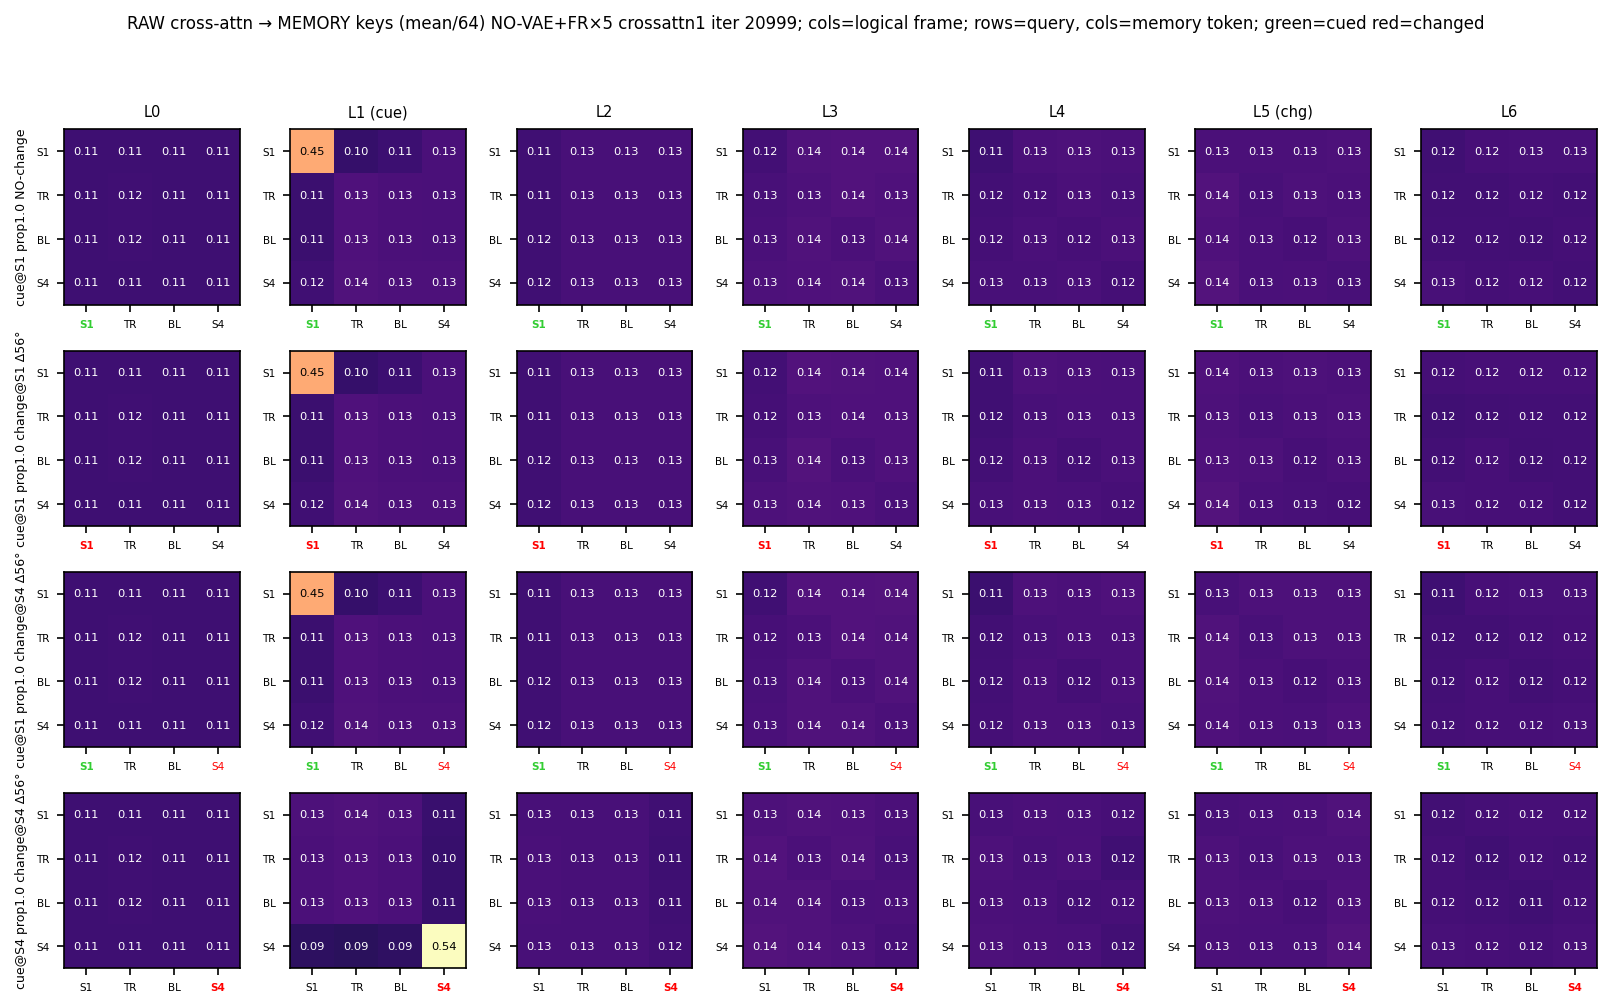
\includegraphics[width=0.78\linewidth]{fr_attn_memory.png}
\caption{\textbf{The frame-repeat pixel route is recurrence-centric.} Memory-key
cross-attention across the $35$ physical frames for the no-VAE frame-repeat model. The
allocation is near-uniform; the only structure is a transient cue-frame read. There is no
change-lock at any memory width --- detection is carried by the recurrent cell, not the
attention weights.}
\label{fig:jepa-fr}
\end{figure}

\section{Result B: the convolutional front-end and its sharp covert-cueing algorithm}
\label{sec:jepa-resultB}
The second route gives the network a \emph{capable per-frame encoder} instead of integration
time. A small SE-ResNet convolutional front-end ($\sim594$K parameters, trained end-to-end,
no VAE checkpoint) processes each $25\times25\times3$ patch through a $3\times3$ stem and
three squeeze-excite residual stages (GroupNorm, SiLU, downsample $25\to13\to7$, channels
$32\to64\to128$), global-average-pools, and emits a $128$-d embedding; the token is
$[\text{emb}_{128}\,\|\,\text{pos}_4\,\|\,\text{temporal}_8]=140$-d. On the plain seven-step
task ($\text{frame\_repeat}=1$, $d_{\text{mem}}=128$) with cross-attention feedback, the JEPA
loss descends from $\sim5.07$ (first-20 mean) to $\sim1.99$ (last-200 mean), a healthy
non-zero plateau, and the network reaches $0.8425$ final / $0.8695$ last-200-mean training
rolling correct. A held-out greedy evaluation at iteration $9{,}599$ (not the final iteration
$12{,}989$) gives correct $0.865$, hit $0.76$, correct-rejection $0.96$, false-alarm
$0.044$, reaction time $5.1\pm0.3$ --- a conservative detector and the only JEPA variant with
a measured greedy number.

Because a strong per-frame encoder solves perception without frame-repeat, the network can
afford an \emph{attention-driven} strategy, and the full mechanism is legible.
\textbf{Psychometric cueing} (Fig.~\ref{fig:jepa-psych}): forced detection rises with change
magnitude and saturates by $44^\circ$; validly cued changes are detected at lower magnitude
than invalid (P(detect) at $16^\circ$ $=0.58$ valid vs $0.43$ invalid; at $28^\circ$ $=0.99$
vs $0.94$), a classic left-shift cueing benefit driven by the spatial cue, not the displayed
validity ring. \textbf{Frame-gating} (Fig.~\ref{fig:jepa-framegate}): cross-attention reads
the image essentially only on the cue frame ($t{=}1$, image-key attention near ceiling) and
runs from memory on every Gabor/change frame (image-key $\approx0$); the current image is
never lost because it enters the cell via the residual $X^{(t)}$. \textbf{Cue-frame read}:
the three non-cued queries place $\sim1.00$ of their attention on the cued image patch,
broadcasting the cue to all four tokens. \textbf{Cue-timed memory change-lock}
(Fig.~\ref{fig:jepa-lock}): valid changes lock at $t{=}5$ (cue@S1 $+0.20$, cue@S4 $+0.24$)
and strongly at $t{=}6$ ($+0.75$, $+0.74$); invalid changes show \emph{no} lock at $t{=}5$
($-0.03$, $-0.02$) and lock only at $t{=}6$ ($+0.70$, $+0.69$) --- the cue buys one frame of
attentional latency, the attentional analogue of the behavioural cueing benefit.
\textbf{Validity/value invariance}: attention allocation is invariant to cue validity
(proportion $0.25$--$1.0$) and cue value (colour); validity and value act downstream at the
decision, a deployment-versus-use dissociation. \textbf{Temporal decoding}
(Fig.~\ref{fig:jepa-decode}): a four-fold cross-validated logistic probe on $\text{vec}(H)$
decodes cue position and value perfectly ($1.00$) from $t{=}1$, while change presence/location
is at chance until the change, then rises to $0.88$/$0.97$ at $t{=}5$ and $0.98$/$0.99$ at
$t{=}6$ --- change is localised in the recurrence at $t{=}5$, one frame before the
invalid-condition attention lock at $t{=}6$, so ``recurrence computes, attention reflects.''
\textbf{Causal memory read} (Fig.~\ref{fig:jepa-causal}): additively suppressing the cued
memory token costs little (P(detect) at $16^\circ$ $0.57\to0.47$); suppressing all four costs
more at high magnitude ($0.98\to0.84$ at $28^\circ$) but does not abolish detection, because
the changed Gabor rides in on the residual $X^{(t)}$. The memory read refines the decision by
$\sim0.1$--$0.15$; it is not the primary change-signal carrier.

\begin{figure}[t]
\centering
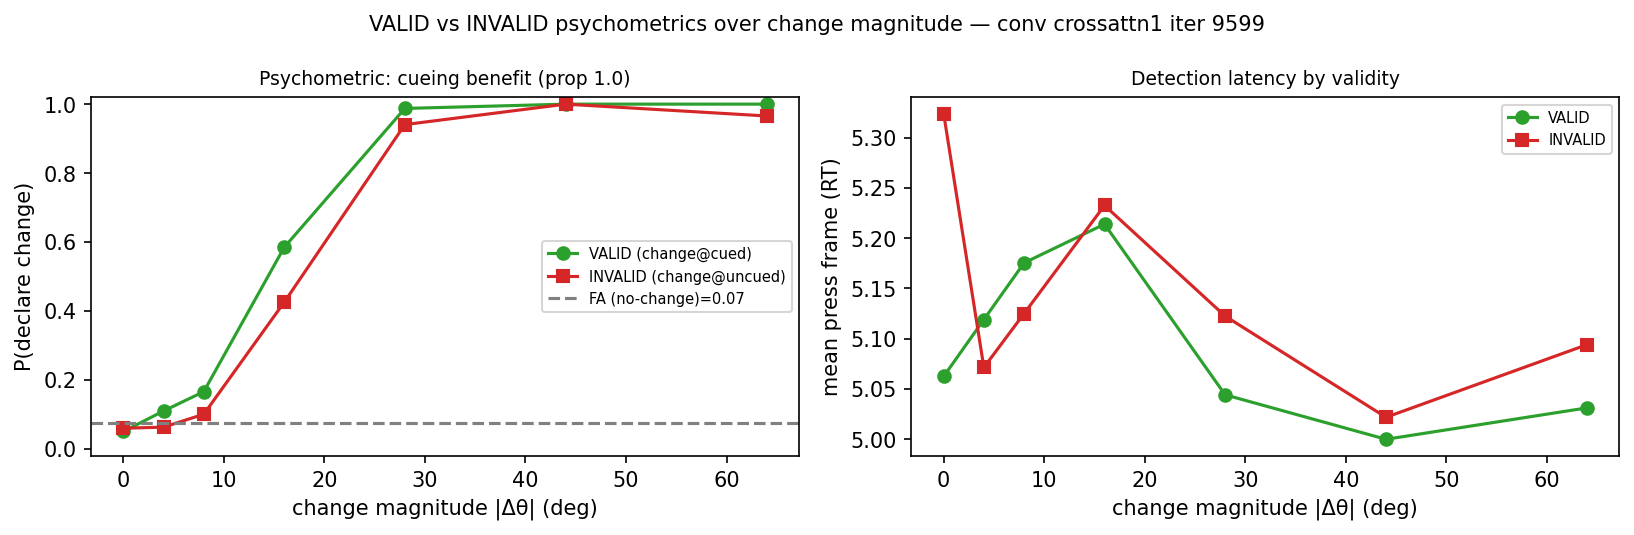
\includegraphics[width=0.62\linewidth]{dd4_psychometric.png}
\caption{\textbf{Psychometric cueing benefit.} P(declare change) versus change magnitude for
validly and invalidly cued changes. Valid cueing left-shifts the curve (e.g.\ $0.58$ vs
$0.43$ at $16^\circ$), saturating by $44^\circ$ --- the behavioural signature of covert
spatial attention.}
\label{fig:jepa-psych}
\end{figure}

\begin{figure}[t]
\centering
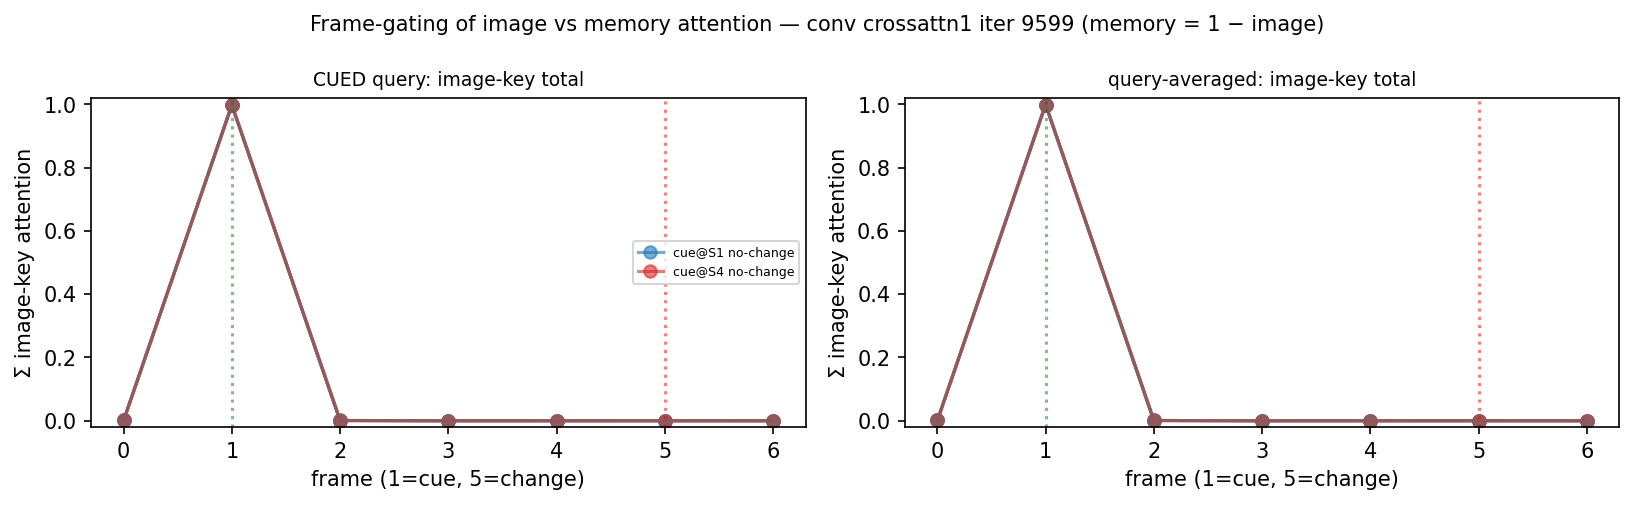
\includegraphics[width=0.72\linewidth]{dd2_framegate.png}
\caption{\textbf{Frame-gated attention.} Summed image-key cross-attention by frame. The
network reads the image only on the cue frame ($t{=}1$) and runs from memory thereafter; the
live image is preserved on the residual.}
\label{fig:jepa-framegate}
\end{figure}

\begin{figure}[t]
\centering
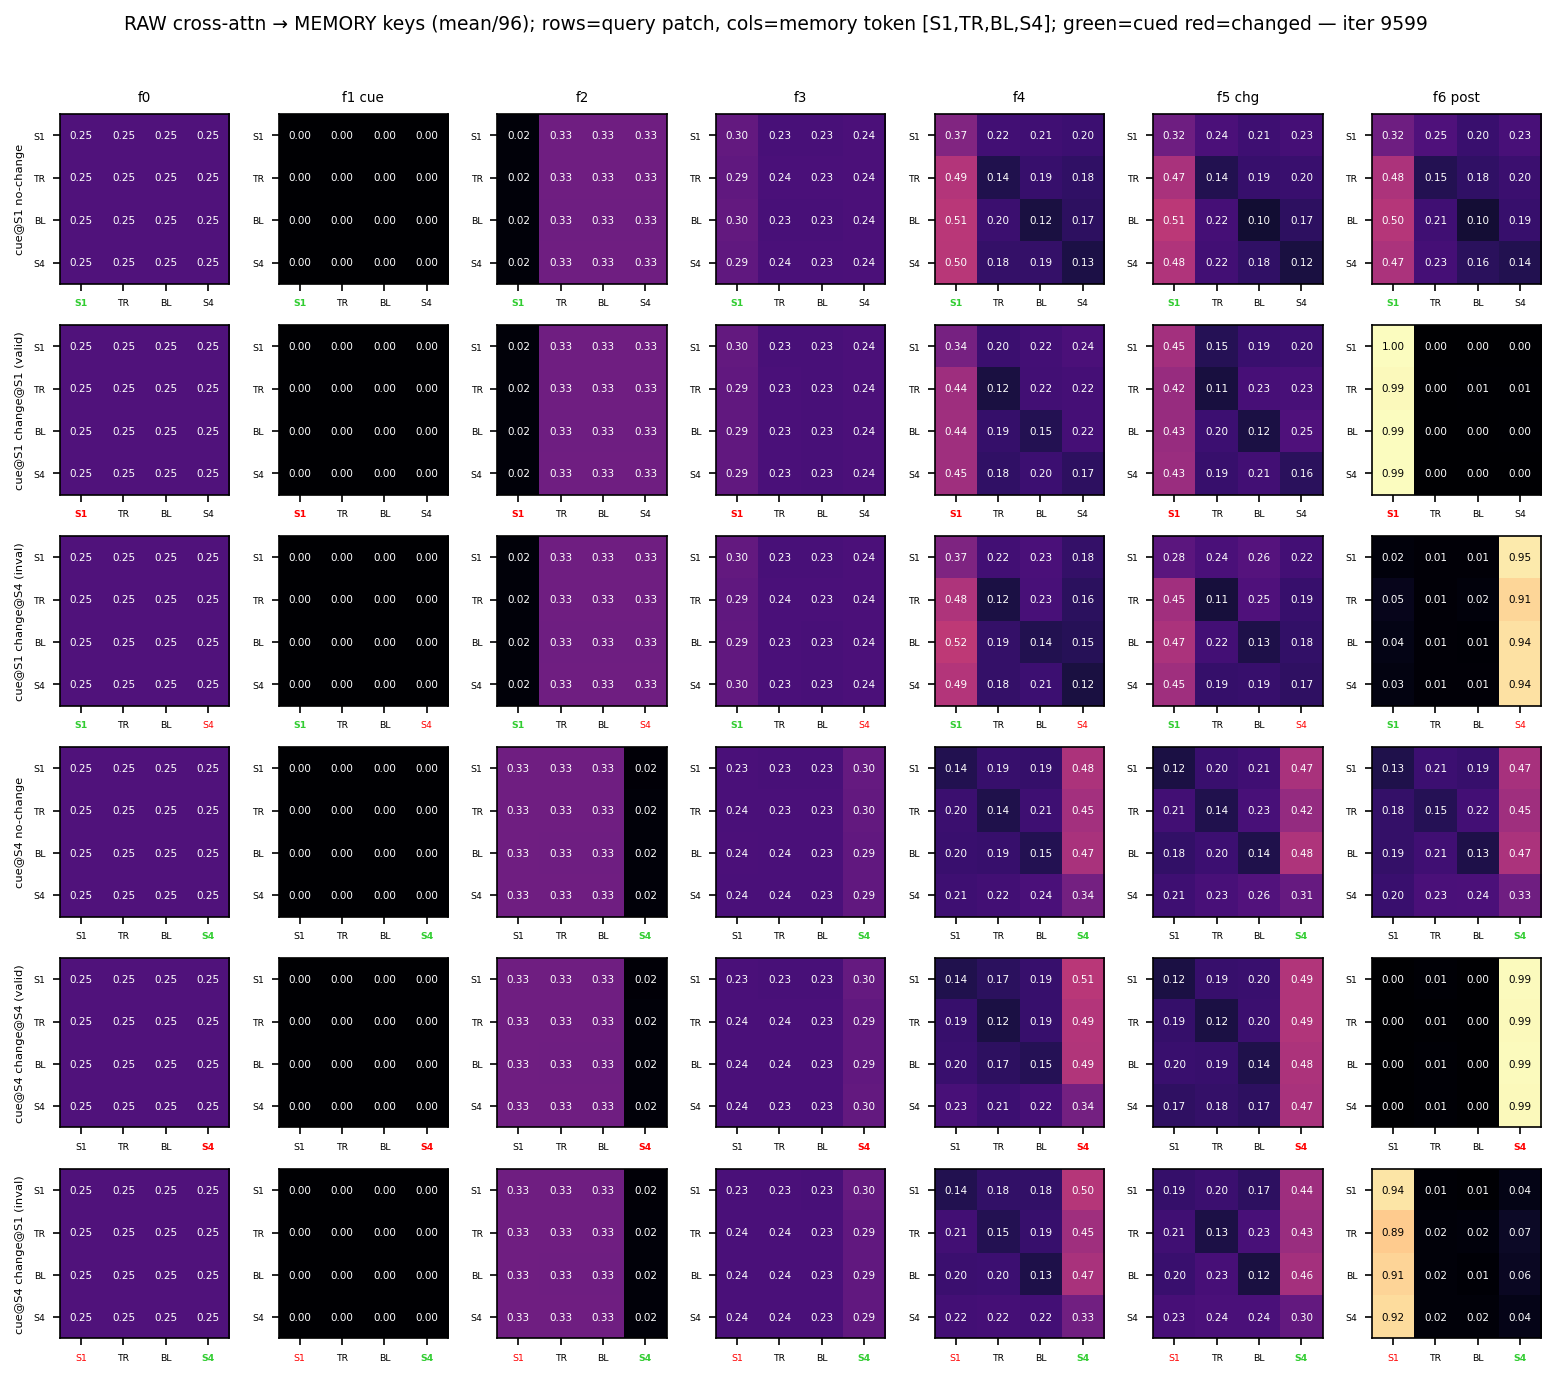
\includegraphics[width=0.82\linewidth]{dd2_maps_memory.png}
\caption{\textbf{Cue-timed memory change-lock.} Memory-key attention maps across frames.
Validly cued changes lock onto the changed location one frame earlier ($t{=}5$) than invalid
($t{=}6$) --- the attentional analogue of the behavioural cueing benefit.}
\label{fig:jepa-lock}
\end{figure}

\begin{figure}[t]
\centering
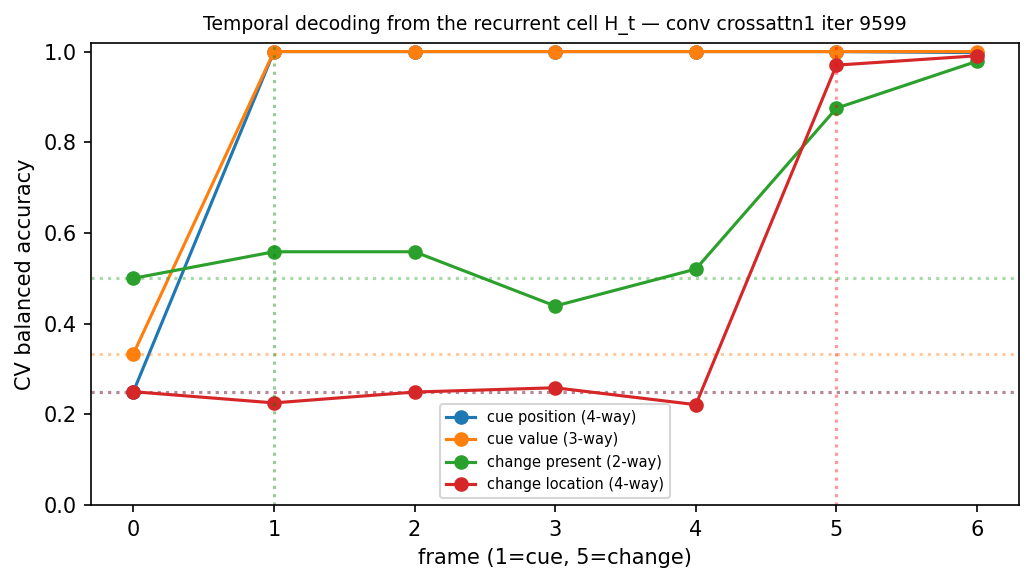
\includegraphics[width=0.62\linewidth]{dd5_decoding.png}
\caption{\textbf{Temporal decoding of the recurrent state.} Cross-validated balanced accuracy
of a logistic probe on $\text{vec}(H)$. Cue position/value are decodable from $t{=}1$; change
presence/location become decodable at $t{=}5$, one frame before the invalid-condition
attention lock --- recurrence computes, attention reflects.}
\label{fig:jepa-decode}
\end{figure}

\begin{figure}[t]
\centering
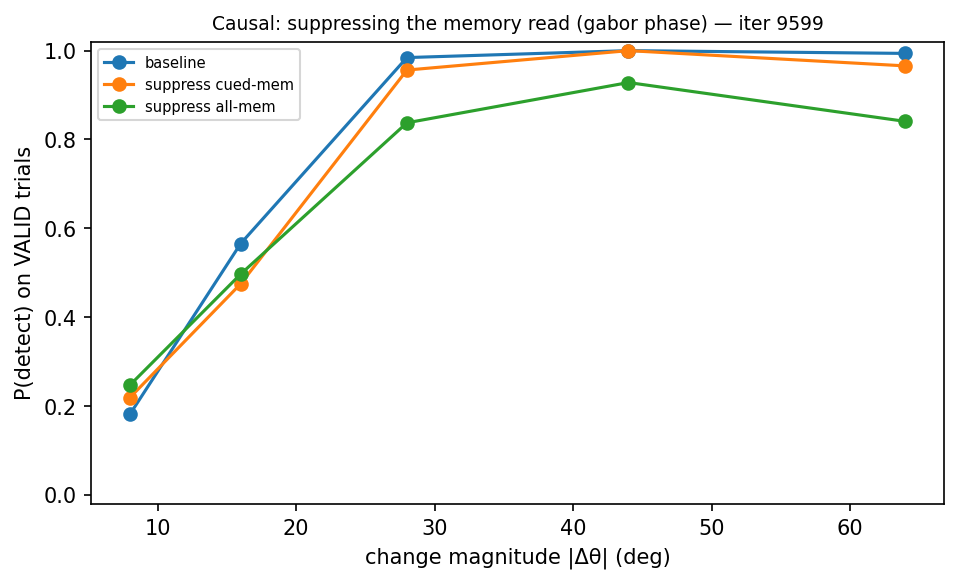
\includegraphics[width=0.62\linewidth]{dd5_causal.png}
\caption{\textbf{Causal perturbation of the memory read.} Additively suppressing memory
tokens on validly cued trials lowers detection modestly but does not abolish it: the changed
Gabor enters on the residual, so the memory read refines rather than carries the change
signal.}
\label{fig:jepa-causal}
\end{figure}

An element-wise-affine feedback variant (modulation $X'=\gamma(H)\odot X+\beta(H)$ then
self-attention over the four image patches, no separate memory-key column) reaches comparable
accuracy ($0.8625$ final / $0.8669$ last-200-mean rolling; greedy $\sim0.83$ at an early
iteration $4{,}199$) but solves the task differently: its change-lock is \emph{bottom-up},
locking onto the changed patch on the change frame for both valid ($1.00$) and invalid
($0.92$) changes --- any large orientation step pulls attention --- which predicts a smaller
cueing benefit. Its attention schedule is orient/release/re-acquire/lock (cued-patch attention
$0.73$ at cue, chance $0.22$ at blank, re-acquiring to $0.80$, saturating $1.0$ at a cued
change). It retains cue position and value at ceiling but \emph{perceives-then-discards} the
validity ring (decoded $0.99$ at $t{=}1$, collapsing to chance by Gabor onset $t{=}3$), the
mechanistic reason its behaviour cannot scale with validity. The two variants are opposite
poles of the same front-end: a memory-timed cueing lock versus a bottom-up salience grab.

\section{Informative negatives: what fences the recipe}
\label{sec:jepa-negatives}
Three negatives establish that the recipe is specific, not a generic ``add a JEPA'' fix.

\textbf{Softmax-as-memory fails.} Externalising the student's per-head softmax $S$
($4\times256=1024$-d) \emph{as} the recurrent memory --- so the same categorical simplex feeds
the cross-attention keys/values, the actor/critic readout, and the JEPA target --- kills task
learning on the no-VAE pixel frame-repeat task. The policy collapses: training rolling correct
peaks early at $0.453$ then decays monotonically to $0$ (late-200 mean $0.0029$). Critically,
the auxiliary itself trains fine (JEPA loss $4.55\to0.48$, a $\sim10\times$ drop, no collapse
to zero), so the failure is a clean dissociation: the representation learns while the policy
fails. A categorical probability simplex is too narrow a working-memory bottleneck; the
continuous cell must remain the working representation.

\textbf{Plain latent-regression JEPA collapses.} A simple SmoothL1 latent-regression auxiliary
(student projects $H2_t$ to predict EMA-teacher $H2_{t{+}1}$; no prototypes, no centring, no
sharpening) on a matrix-affine two-LSTM network exhibits the textbook latent collapse: the loss
falls from $0.489$ to $\sim0.11$ early in training, reaches a minimum of $0.00118$, and pins
near zero (late-2000 mean $0.0828$). With the predictor finding a near-constant target, the
auxiliary supplies no task signal and the policy sits at chance (late-200 mean rolling correct
$0.4975$, final $0.465$). This is the direct justification for the prototype-softmax/DINO-style
machinery in Results~A and~B: the anti-collapse apparatus is what makes the predictive
auxiliary useful.

\textbf{The collapse is the wiring, not the stabiliser.} The same matrix-affine two-LSTM
network collapses to always-wait chance under a \emph{VAE} as well (late-200 mean rolling
correct $0.4963$, final $0.45$). The JEPA did not rescue a wiring that fails regardless of
front-end stabiliser, so the fault is the matrix-affine two-LSTM feedback itself --- not
``affine'' in general, since the element-wise affine variant of Result~B reaches $\sim0.86$.
The negatives jointly localise the requirements: a continuous working memory, genuine
anti-collapse machinery in the auxiliary, and a feedback wiring that learns at all.

\section{Set-size-9 generalization (in progress)}
The conv-JEPA recipe is being carried from the four-stimulus $2\times2$ grid to a harder
nine-stimulus $3\times3$ grid (vda9: $75\times75$ image, coloured value cue, validity ring,
cue positions top-left/bottom-right). Both feedback wirings are above chance early and still
climbing. As of the current frontier (cross-attention at $\sim361$ iterations, element-wise
affine at $\sim353$), training rolling correct is $0.65$ (last-200 mean; $0.695$ final) for
cross-attention and $0.74$ (last-200 mean; $0.803$ final) for element-wise affine; the affine
variant showed an early JEPA descent (minimum $\sim2.46$ near iteration $94$) but the loss has
since risen back toward $\sim3.4$, so auxiliary engagement is not yet established for either
wiring at this set size. These are early, non-converged numbers --- a flat-looking curve this
early is not a ceiling --- so the result is reported as preliminary evidence that the no-VAE
conv-JEPA recipe transfers to the larger set size, not as a final accuracy.

\section{Cross-cutting lesson: architecture sets the attention strategy}
The two working routes reach comparable competence by opposite mechanisms, and the difference
is set by the \emph{perceptual front-end and the task temporal structure, not by memory size}.
A strong per-frame convolutional encoder (Result~B) lets the network afford an attention-driven
solution: a sharp, frame-gated algorithm that orients to the cue once, encodes it, monitors
from memory, and re-points to a change, with a cue-timed memory lock that yields a one-frame
attentional cueing benefit. Learning from held raw pixels (Result~A) instead yields a diffuse,
recurrence-centric solution in which the attention weights carry little structure and detection
lives in the LSTM. The $d_{\text{mem}}$ sweep confirms memory width is not the lever: accuracy
is non-monotonic in it. This sharpens the Chapter~\ref{ch:attention} reading that what carries
the computation --- attention versus recurrence --- is decided upstream of the memory.

For Chapter~\ref{ch:recommendation}, the consequence is a qualification, not a reversal. The
frozen pretrained VAE remains the simplest, most reliable, and best-characterised way to satisfy
the perception requirement, and remains the right default for the empirical manuscript. But the
requirement is now correctly stated as \emph{a front-end that reliably encodes the task
variable}, which can be met either by a frozen pretrained VAE \emph{or} by a self-supervised
predictive auxiliary (with proper anti-collapse machinery) paired with an enabler --- frame-
repeat or a capable conv encoder. The neuro relevance reinforces why this matters:
predict-the-future-latent self-supervision is arguably a more biologically plausible route to a
working visual front-end than supervised reconstruction-pretraining, so the JEPA route is not
merely an engineering alternative but the more defensible model of how a cortical front-end might
come to see.

\chapter{Reinforcement-learning harness variations}
\label{ch:harnessvar}

The harness is held constant across architectures, but several of its knobs are
themselves objects of study, because the deceptive $0.5$ floor of the seven-step task makes
the optimisation as much a part of the result as the network.

\section{Discount and horizon}
The discount $\gamma$ is matched to the horizon: $\gamma=0.95$ for the seven-step task and
$\gamma=0.98$ for the twenty-nine-step task, where credit must travel further from the
change to the cue. These are not finely tuned; the qualitative behaviour is robust across a
band, but a higher $\gamma$ on the longer task does help the cue's effect survive the delay.

\section{Critic particles}
The number of distributional ``particles'' (quantiles, or categorical atoms in the paper's
form) was varied from the published $15$ down to $5$. Fewer particles is a coarser value
distribution; on this low-bandwidth task the value differences the critic must resolve are
small (the gap between ``press now'' and ``wait'' near threshold), so particle count is a
genuine knob rather than a free choice. We default to $5$ for the short task and have run
$15$ on the long task; a systematic sweep is an open item.

\section{Target network: EMA versus hard copy}
The original working checkpoints used a periodic hard-copy target. The reproduction adds an
exponential-moving-average target ($d=0.995$). Whether the EMA helps, hurts, or is neutral
on this task is genuinely open: the working multiplicative$+$VAE model used EMA, but so
would a hard-copy version, and we have not isolated the difference. Because the lab's
canonical working models used the hard-copy target, an EMA-versus-hard-copy A/B on the
frozen-VAE base is on the near-term list --- it is a candidate, alongside the attention form
and head count, for any residual difference between our reproduction and the lab's other
networks.

\section{Exploration and the two collapses}
The recurring optimisation failure is collapse to a $0.5$ optimum, in one of two faces:
always-wait (never press) or always-press-at-the-deadline (press every trial at the change
frame). Both have policy entropy at zero and zero policy gradient --- the actor is frozen,
even while the critic keeps learning the $0.5$ value perfectly. The levers that matter are
maintaining exploration (entropy floor or coefficient, the burn-in length, the initial
action bias) and, decisively, fixing perception (Chapter~\ref{ch:perception}): once the
front-end can see the change, the discriminating policy is reachable and the collapse is
escaped. The lesson for the harness is that an apparently dead run is usually a perception
or exploration problem, not a critic problem.

\section{A resume footgun, fixed}
A practical note that cost real training time: the trainer's \code{resume} mode silently
no-ops if no explicit checkpoint path is set, starting fresh and discarding progress. This
was hardened in both trainers to auto-discover the latest checkpoint in the run directory
and to error loudly when \code{resume} finds nothing, rather than silently restarting.
Checkpoints live outside the synced repository to avoid mid-run corruption.

\chapter{Where this leaves us: an architecture recommendation}
\label{ch:recommendation}

This chapter turns the findings into a recommendation for the network to carry into the
empirical manuscript and to standardise on for the cross-task generalisation goal. We state
the decision criteria, score the candidates against them, and give a contingent
recommendation that names what must be resolved before it is final.

\section{Decision criteria}
A network is a good choice for this program to the extent that it:
\begin{enumerate}
\item \textbf{reproduces the behavioural signatures} --- the reliability-scaled cueing
benefit and the causal attention-to-sensitivity link (Chapter~\ref{ch:deepdive});
\item \textbf{exposes an interpretable, causally manipulable attention signal} --- the
attention must be readable and a genuine lever on behaviour (the microstimulation-like
causal result, Chapter~\ref{ch:deepdive}). Note the matched family showed that on the
short task the cueing itself is carried by \emph{memory}, not expressed as a cue-orienting
map (Chapter~\ref{ch:attention}), so this criterion is about a manipulable attention
\emph{lever}, with cue-orienting treated as a regime-dependent property, not a requirement;
\item \textbf{generalises across the task battery} (validity, set-size, value, distractor,
reward-structure) with the same architecture and harness;
\item \textbf{is neuro-plausible} --- recurrent gain modulation, a capacity-limited working
memory, reward-driven learning, and a manipulable priority signal; and
\item \textbf{trains reliably} under the stable harness with the frozen-VAE front-end.
\end{enumerate}

\section{Two non-negotiables}
Two components are settled by the evidence and should be fixed regardless of the remaining
choices. First, the \textbf{frozen pretrained VAE front-end} (Chapter~\ref{ch:perception}):
perception cannot be learned from reward by supervised reconstruction on the short task, the
VAE is task-parameter-invariant, and freezing it makes architecture comparisons clean.
Chapter~\ref{ch:jepa} shows the requirement is more precisely \emph{a front-end that reliably
encodes the task variable}, satisfiable by a frozen pretrained VAE \emph{or} by a
self-supervised V-JEPA predictive auxiliary (with anti-collapse machinery) paired with
frame-repeat or a convolutional encoder; the frozen VAE remains the recommended default for
the empirical manuscript on grounds of simplicity and characterisation. Second, the \textbf{stable
harness} --- PAC actor, distributional critic, prioritised episode replay, a time-lagged
target, and burn-in --- which is what makes a bootstrapped recurrent actor--critic learn on
a task with a $0.5$ harbor.

\section{The attention-mechanism choice (now decided)}
The matched family (Chapter~\ref{ch:attention}, Table~\ref{tab:familyresults}) was built to
settle this, and it did --- by eliminating the premise that one wiring would restore
cue-orienting attention. Reading the family against the criteria:
\begin{itemize}
\item The \textbf{pure multiplicative single-stream} form is the most faithful to the
published equation and reproduces the behaviour (correct $0.804$, hit $0.705$); its
attention is change-locked (spike $+0.143$, orient $\approx0$). On the new criterion (2) it
passes --- the attention is a readable, causally manipulable change detector --- it simply
does not orient to the cue, which the family shows \emph{nothing} on this task does.
\item The \textbf{two-LSTM} variant is the same paper-faithful multiplicative attention with
a second stacked memory feeding the heads, and it is the \emph{best detector in the family}
(correct $0.872$, hit $0.836$), while keeping the same interpretable, change-locked,
causally-manipulable attention. It is the strongest candidate on criteria (1), (4), (5) and
the new (2), at a minimal, well-motivated departure from the published network.
\item The \textbf{cross-attention} and \textbf{dual-memory} variants work (correct $0.840$,
$0.828$) but attend \emph{below} uniform at the cued image location (cue-orient $-0.179$,
$-0.174$): they route processing through memory keys rather than the image, which neither
helps behaviour over two-LSTM nor yields the cue-orienting map the lineage showed on the
older long-task setup. The earlier expectation that cross-attention would orient here was
not borne out on the controlled frozen-VAE short-task base.
\item The \textbf{affine} modulation \emph{failed} (always-wait collapse, hit $0$); it is
out. The \textbf{dual-head} sensory head is the only positive cue-orient ($+0.038$) but far
too weak to feature.
\item The \textbf{split priority/value (cross-talk)} architecture remains the vehicle for
mechanistic dissociations (Chapter~\ref{ch:crosstalk}); its $\mu/q$ mapping onto anatomy is
delicate, and the empirical paper's scope (per James) excludes architecture variants. It is
the subject of a \emph{separate} paper, not the recommended manuscript network.
\end{itemize}

\section{Recommendation}
\textbf{For the empirical manuscript:} a single-stream recurrent vision transformer with
(i) the frozen pretrained VAE front-end, (ii) the \textbf{multiplicative recurrent attention
block with a second stacked xLSTM memory} (the \code{two-lstm} variant) --- the best detector
in the matched family and a minimal, paper-faithful change to the published equation ---
(iii) a spatial xLSTM working memory, and (iv) a distributional actor--critic readout,
trained by the stable harness across the full task battery. This satisfies criteria
(1), (3), (4), (5) and the reframed (2): the attention is interpretable and a causal lever
on sensitivity, while the cueing benefit is carried, honestly and demonstrably, by working
memory.

The accompanying scientific claim is that, on the seven-step task, \textbf{the cueing
benefit is memory-borne and the attention map is a bottom-up change detector} --- a result
now established across six wirings, not assumed. The manuscript's attention figure should
therefore be the \emph{causal} one (biasing attention shifts sensitivity, with no induced
false alarms; Chapter~\ref{ch:deepdive}), not a cue-orienting map the mechanism does not
produce. Whether a longer delay or harder cue \emph{forces} pre-orienting --- as the lab's
older long-task networks displayed --- is a regime question to test with this same network,
not a reason to change the architecture.

\textbf{For the separate architecture line:} the split priority/value cross-talk network is
the vehicle for the coupling-required and double-dissociation results --- a strong paper in
its own right, kept out of the empirical manuscript by design.

\section{What must be resolved before this is final}
The attention-mechanism question is now settled; what remains: (1) the chosen network
(\code{two-lstm}) must be shown to generalise across at least the value (\code{vda4}) and
set-size (\code{setsize9}) tasks with no architecture change; (2) the cross-talk coupling
result must be replicated on the short task with the frozen VAE to confirm it survives the
perception fix; and (3) the regime question --- does a longer delay restore cue-orienting
attention in the recommended network? --- should be tested, since it bears on whether the
published orienting figure is reproducible at all in our setup or is specific to the long
task. Frozen VAE, the stable harness, and now the two-LSTM multiplicative attention are
fixed; the open items are generalisation and two targeted controls.

\chapter{Proposed experiments}
\label{ch:experiments}

The experiments fall into two tracks: the \emph{task-battery expansion} that broadens the
empirical manuscript (per James's plan), and the \emph{architecture experiments} that close
the open mechanistic questions. Both run on the recommended network
(Chapter~\ref{ch:recommendation}) so that results compose.

\section{Track 1 --- the task battery (empirical manuscript)}
The goal is to show one architecture, one harness, reproducing primate signatures across
the standard battery --- the direct answer to the first submission's ``limited in scope.''

\paragraph{Visual-discrimination / value-cue (\code{vda4}).} The cue colour sets reward
magnitude ($5/3/1$). The prediction: behaviour is graded by value as well as by spatial
validity, and the critic's value estimates are calibrated and ordered by reward. This adds
the value-direction axis to the spatial-cueing axis and exercises the reward-driven-learning
differentiator.

\paragraph{Set-size (\code{setsize\{2,4,9\}}).} The nine-stimulus task with five validity
levels (including an uninformative $0$) tests whether the cueing benefit \emph{grows} with
set size. This is the empirical bridge to the normative set-size/accidental-hit theory
(Paper B): the prediction that the uncued-false-alarm benefit trades off at $K=2$ and flips
positive at $K=4$ should have a behavioural correlate in the model. \textbf{Must be run on
the canonical architecture}, not the cross-talk variant, and with the frozen VAE.

\paragraph{Reward structure (Luo \& Maunsell).} Sensitivity-versus-criterion sessions after
Luo \& Maunsell (2018), decomposing performance into $d'$ and criterion. The model should
reproduce the dissociation between reward-driven sensitivity changes and criterion shifts.

\paragraph{Attend / ignore (Krauzlis).} An uncued change that must be actively ignored. The
distractor result from \code{v11\_part5} (the distractor is filtered in the decision pathway
while remaining decodable from sensory memory --- ``seen but not acted upon'') is the
prediction to replicate on the canonical network.

\paragraph{Discrimination (Baruni, optional).} A discrimination variant to round out the
battery if the reviewers want a non-detection task.

\section{Track 2 --- the architecture / mechanism experiments}
\paragraph{The cue-attention question (\emph{done}).} The matched family
(\code{multiplicative}, \code{dualhead}, \code{two-lstm}, \code{crossattn}, \code{dualmem};
\code{affine} collapsed) was trained on the frozen-VAE base and the cue-$100\%$ change/
no-change attention contrast run on each (Chapter~\ref{ch:attention},
Table~\ref{tab:familyresults}). Outcome: no wiring restores cue-orienting attention on the
short task; \code{two-lstm} is the best detector and the recommended network. The follow-up
(O5) is the longer-delay regime test below.

\paragraph{The optic-flow reaction-time test.} Directly compare reaction-time distributions
of the from-scratch long-task model (predicted late, integrating) against the pretrained-VAE
short-task model (predicted early, perceiving). This is the falsifiable test of the
horizon/strategy theory (Chapter~\ref{ch:horizon}) and needs no new training --- only
analysis of existing checkpoints.

\paragraph{Coupling on the short task.} Replicate the coupling-required result
(Table~\ref{tab:crosstalk}) on the seven-step task with the frozen VAE, to confirm it
survives the perception fix and is not an artefact of the long-horizon flow regime.

\paragraph{EMA-versus-hard-copy A/B.} Isolate whether the target-update rule is one of the
residual differences between our reproduction and the lab's canonical working networks.

\paragraph{The representational and causal dissociations.} On a trained value-task network,
decode change-evidence versus value/context from the two streams (representational
dissociation), and run the $\mu$-clamp / $q$-clamp causal battery (decision collapses under
$\mu$-clamp; value-modulation degrades but detection is spared under $q$-clamp). These are
the paper-worthy claims of the separate architecture line.

\section{Sequencing and cost}
The analysis-only experiments (optic-flow reaction time, the matched-family attention
contrast once checkpoints land) are cheap and come first. The battery retrains are the bulk
of the compute and should be run one at a time on the available accelerator, reusing the
single frozen VAE across all of them (Chapter~\ref{ch:perception}). The set-size and value
tasks are the highest-value additions for the empirical manuscript and should lead.

\chapter{Research plan}
\label{ch:plan}

The plan is staged so that each stage produces a decision or a deliverable, and so that the
cheap, decisive analyses precede the expensive retrains. It serves two outputs in parallel:
the empirical manuscript (Paper A) and the separate architecture/dissociation paper.

\section{Stage 0 --- settle the network (\emph{largely done})}
\begin{itemize}
\item \textbf{Done:} the matched attention family is trained on the frozen-VAE base and the
cue-attention contrast is run on each (Chapter~\ref{ch:attention}). The decision is made ---
\textbf{the recommended network is the \code{two-lstm} multiplicative form}, the best
detector in the family; \code{affine} collapsed and no variant orients to the cue, so the
cueing story is memory-borne and the manuscript's attention figure is the causal one.
\item Run the optic-flow reaction-time analysis on existing checkpoints (no new training).
\item Run the EMA-versus-hard-copy A/B to close the last reproduction-difference question.
\item Test the longer-delay regime (O5) on \code{two-lstm} --- does any delay restore
cue-orienting attention, or is the published orienting figure long-task-specific?
\item \emph{Deliverable:} a single, named recommended network (frozen VAE $+$ two-LSTM
multiplicative attention $+$ stable harness) --- the architecture every subsequent run uses.
\end{itemize}

\section{Stage 1 --- generalisation across the battery ($\sim$2--3 weeks)}
\begin{itemize}
\item Train the recommended network, unchanged, on \code{vda4} (value) and
\code{setsize9} (set-size) first, then \code{luo\_maunsell} and \code{krauzlis}.
\item For each, run the standard analysis suite: psychometric/chronometric fits,
attention maps, the causal attention battery, and (for the value tasks) critic calibration.
\item \emph{Deliverable:} the empirical manuscript's results section --- one architecture,
one harness, reproducing primate signatures across the battery, with per-validity
breakdowns and the corrected attention-map visualisation.
\end{itemize}

\section{Stage 2 --- the causal-prediction differentiators ($\sim$2 weeks)}
\begin{itemize}
\item Formalise the causal-perturbation predictions (attention clamps mapping onto SC/FEF
microstimulation and inactivation) as the manuscript's novel contribution, alongside the
reward-driven-learning differentiator.
\item Run the representational decoding (change-evidence vs.\ value/context) to support the
predictions.
\item \emph{Deliverable:} the manuscript's discussion/predictions section and the
``NN-steers-neuroscience'' framing carried implicitly by the predictions.
\end{itemize}

\section{Stage 3 --- the architecture / dissociation paper (parallel track)}
\begin{itemize}
\item Replicate the coupling-required and swapped-routing results on the short task with the
frozen VAE; run the $\mu$/$q$ representational and causal double-dissociation.
\item Position as a separate paper: ``coupling between policy and value is required for
attentive behaviour to be learned,'' with the double dissociation as the headline.
\item \emph{Deliverable:} the architecture paper draft (the existing cross-talk manuscript
is the seed).
\end{itemize}

\section{Stage 4 --- the normative theory preprint (James first author, parallel)}
\begin{itemize}
\item The set-size/accidental-hit normative result (uncued-FA benefit flips with set size),
cited by the empirical paper, on a fast venue.
\item The model's set-size behaviour (Stage 1) provides the empirical correlate.
\end{itemize}

\section{Risks and contingencies}
\begin{itemize}
\item \emph{No matched variant restored cue-orienting attention on the frozen-VAE base (the
realized case):} this is now a positive result --- on the seven-step task the cueing benefit
is memory-borne across all six wirings --- and the manuscript features the causal attention
result with the memory-driven account stated plainly, rather than a cue-orienting map the
mechanism does not produce. The residual risk is O5: if a longer delay never restores
orienting either, the published orienting figure may be specific to the long-task regime,
which is itself a reportable finding.
\item \emph{If the network fails to generalise to a battery task:} treat the failure as a
diagnostic (perception, exploration, or coupling, per the lessons of
Chapters~\ref{ch:perception}--\ref{ch:crosstalk}) rather than a reason to fork the
architecture; the generalisation goal is the point.
\item \emph{Compute:} runs are serialised on the available accelerator, one frozen VAE is
reused across all tasks, and analysis is thread-capped and run only when training is idle ---
the laptop has been crashed once by stacking compute, and that constraint is now hard.
\end{itemize}

\chapter{Summary of findings}
\label{ch:findings}

This chapter collects the load-bearing findings in scannable form --- the things that are
established and should carry forward, separated from the things that are still open.

\section{Established findings}

\paragraph{F1. Perception is the bottleneck on the short task.} A front-end trained from
reward alone cannot represent orientation (linear orientation decodability $\Rsq=0.24$);
a reconstruction-pretrained VAE encoder reaches $\Rsq=0.97$, and with that single change the
exact paper network learns the seven-step task on the first attempt. \emph{Action:} use a
frozen pretrained VAE front-end; fix perception before comparing architectures.

\paragraph{F2. One VAE serves all task variants.} The VAE is a static, per-frame encoder;
the temporal task parameters ($\sigma$, horizon $T$) do not change its input distribution.
\emph{Action:} pretrain one VAE and reuse it across all noise levels and horizons --- do not
re-pretrain per task.

\paragraph{F3. The horizon decides the strategy.} The long task is solvable by slow temporal
integration (``flow''), which tolerates a weak front-end; the short task forecloses flow and
forces instantaneous perception. This explains why the VAE is necessary on the short task
and not the long one. \emph{Action:} use the short task as the discriminating test bed; use
the long task to study maintenance/anticipation.

\paragraph{F4. Coupling is a precondition for learning.} Severing the shared recurrent
memory between the policy and value streams collapses an otherwise identical model from
$0.87$ accuracy to chance; routing the memory-grounded stream (instead of the grounded
stream) to the policy also collapses it. \emph{Action:} keep a shared substrate coupling
value to action, and let the grounded, image-reading stream drive the policy.

\paragraph{F5. Routing decides the phenotype, not representation.} Identical encoders yield a
working detector or a chance model depending only on which stream drives the policy and
whether a shared memory couples value to action.

\paragraph{F6. A grounded image pathway is required.} Every variant that removes the
bottom-up route to memory or to the decision collapses to always-wait. \emph{Action:} never
fully bottleneck visual information through memory.

\paragraph{F7. The working model reproduces the paper's behaviour.} On the seven-step task
with a frozen VAE: a reliability-scaled cueing benefit ($+1.5^\circ\!\to\!+7.5^\circ$ across
$25\%\!\to\!100\%$ validity, carried by the sensitivity threshold) and a causal
attention-to-sensitivity link ($+8.5\%/-8.0\%$ from biasing attention toward/away from a
change, with no induced false alarms).

\paragraph{F8. The cueing effect is memory-driven, across the whole family.} In the
multiplicative-gated model the cue and its validity are held in working memory ($100\%$
decodable) and set the decision criterion, while the attention map stays change-locked. The
matched family (\code{multiplicative}, \code{dualhead}, \code{two-lstm}, \code{crossattn},
\code{dualmem}; \code{affine} collapsed) confirms this is \emph{general}: no working variant
produces a cue-orienting index above $+0.04$, and the two richest cross-talk wirings attend
\emph{below} uniform at the cued image location ($-0.18$), routing the cue through memory.
\emph{Action:} read the attention maps with this dissociation in mind; do not assume cue use
implies cue-orienting attention; feature the causal attention result, not a cue-orienting
map, on the short task.

\paragraph{F9. The harness is a stable recipe with two failure harbors.} PAC actor,
distributional critic, prioritised episode replay, a time-lagged target, and burn-in train a
bootstrapped recurrent actor--critic on this task. The recurring failures are two $0.5$
collapses (always-wait and always-press-at-deadline); both are perception/exploration
problems, not critic problems. \code{affine} (matrix scale $+$ shift) fell into the
always-wait harbor and never recovered ($P(\text{press})\le0.004$), a reminder that not
every modulation form trains.

\paragraph{F10. Two stacked memories is the best detector, and the recommended network.}
Across the matched family on the identical frozen-VAE base, the \code{two-lstm} variant ---
the published multiplicative attention with a second stacked xLSTM feeding the heads --- is
the best detector (correct $0.872$, hit $0.836$ vs.\ $0.804/0.705$ for the plain
multiplicative form), while preserving the interpretable, change-locked, causally
manipulable attention. \emph{Action:} carry \code{two-lstm} forward as the manuscript
network; feature the causal attention result, not a cue-orienting map.

\paragraph{F11. Perception is learnable without a pretrained VAE.} A jointly-trained V-JEPA
temporal self-distillation auxiliary (prototype-softmax, EMA teacher, student$@t\!\to$
teacher$@t{+}1$) learns a working front-end from raw pixels with frame-repeat ($\sim0.90$
training rolling correct) or with an SE-ResNet convolutional encoder ($\sim0.87$ greedy
correct, with a sharp attention-driven covert-cueing algorithm) --- no pretrained or frozen
VAE. Negatives fence the recipe: softmax-as-memory and a plain SmoothL1 latent JEPA collapse,
and the matrix-affine two-LSTM wiring collapses regardless of front-end. This qualifies F1 and
the Chapter~\ref{ch:recommendation} non-negotiable (Chapter~\ref{ch:jepa}). \emph{Action:}
keep the frozen VAE as the manuscript default; hold the JEPA route as the neurally-plausible
alternative and a set-size/battery generalisation vehicle.

\section{Open questions}

\paragraph{O1. \emph{(Resolved.)} Which wiring restores cue-orienting attention?} None do, on
the seven-step task. The matched family (\code{multiplicative}, \code{dualhead},
\code{two-lstm}, \code{crossattn}, \code{dualmem}; \code{affine} collapsed) shows the cueing
effect is memory-borne across all working wirings (cue-orient $\le+0.04$; \code{crossattn}
and \code{dualmem} attend \emph{away} from the cued image patch). The remaining version of
the question is now O5: whether a \emph{longer-delay} regime forces orienting.

\paragraph{O2. Does the coupling result survive the perception fix?} The
coupling-required result was obtained on the long task before the VAE finding; replicating
it on the short task with the frozen VAE is pending.

\paragraph{O3. Is the EMA target load-bearing?} An EMA-versus-hard-copy A/B on the
frozen-VAE base will close the last difference between our reproduction and the lab's
canonical working networks.

\paragraph{O4. Does the chosen network generalise across the battery?} The value and
set-size tasks are the first generalisation tests; failure on any is to be read as a
diagnostic, not a reason to fork the architecture.

\paragraph{O5. Does a longer delay restore cue-orienting attention?} The published lab
networks (long task) displayed cue-orienting attention; our short-task family does not. This
is plausibly a regime effect (a longer cue--target delay may make pre-orienting worth its
cost) rather than an architecture effect. Running the recommended \code{two-lstm} network on
a longer-delay variant tests whether the published orienting figure is reproducible at all
in our setup, and connects directly to the optic-flow account (Chapter~\ref{ch:horizon}).

\section{Reusable infrastructure}
The program leaves a reusable substrate: a single clean \code{ChangeDetectionEnv} with a
task registry (validity, value, set-size, distractor, reward-structure, attend/ignore); a
shared PAC$+$QR-DQN$+$PER harness with hard-copy and EMA targets; a pretrained, frozen,
task-invariant VAE front-end; a \code{--feedback} switch that selects among seven attention
mechanisms on the identical base; and an analysis suite (psychometric/chronometric fits,
attention maps, causal attention clamps, representational decoding) that runs from saved
data without re-loading models.

\chapter{Conclusion}
\label{ch:conclusion}

The program set out to find a single, neuro-inspired recurrent vision transformer that
learns covert spatial attention from reward, reproduces primate signatures, and generalises
across tasks. After roughly thirty variants and two task horizons, the picture is clearer
than the variant count suggests, because the results collapse onto a few principles.

\textbf{Perception comes first.} The most expensive lesson was the cheapest to fix: sparse
reward cannot teach a front-end to see orientation, and a reconstruction-pretrained VAE
solves it outright. Much of the earlier difficulty on the short task was perception failing
in an architecture's clothes, and separating the two questions --- can it see, and is it
wired right --- is the methodological gain that makes the rest of the comparisons clean.

\textbf{The horizon is a design variable.} The same task at two lengths admits two different
solutions, and recognising that the long task hides perception failures behind temporal
integration explains a paradox that had stalled the program. The short task, with the cue's
information forced through memory and the change forced through perception, is the sharper
instrument.

\textbf{Wiring decides the phenotype.} Coupling value to action through a shared memory is a
precondition for learning, not an optimisation; a grounded image pathway is required; and
which stream drives the policy matters as much as what the streams represent. These routing
facts, not any single clever module, are what separate the models that learn from the models
that collapse.

\textbf{The model already reproduces the paper, and the matched family settled the
mechanism.} With perception fixed, the network reproduces the reliability-scaled cueing
benefit and the causal attention-to-sensitivity link. It also surfaced a genuine mechanistic
question --- a cueing effect carried by memory rather than by attention orienting --- which
the matched family of six wirings has now resolved: \emph{no} variant orients to the cue on
the short task, so the effect is memory-borne in general, not a quirk of one gate. The same
sweep named the network: the two-LSTM multiplicative form is the best detector and a
minimal, paper-faithful choice.

What remains is execution: with the attention mechanism settled and the frozen VAE and
stable harness fixed as constants, run that one architecture across the task battery, and
test whether a longer-delay regime ever restores the published cue-orienting figure. That is
the path from a zoo of variants to the single, interpretable, generalising model the program
was after --- and to an empirical manuscript whose figures, behavioural and neural, are
produced by the same network, with a cueing mechanism reported as it actually is.


\nocite{*}
\bibliography{refs}

\appendix
\chapter{Per-model atlas: architecture, attention, and behaviour}
\label{app:atlas}

This appendix gives, for \emph{every} trained variant, three things on one or two pages: a
diagram of its architecture, its attention maps at every time point, and its psychometric and
chronometric functions. All models share the frozen pretrained VAE front-end, the
PAC$+$QR-DQN$+$PER harness, and the $4096$-d flattened-memory readout; they differ only in the
attention/memory wiring drawn in each diagram.

\paragraph{How to read the attention maps.} Each attention figure forces the agent to wait so
the full seven-frame timecourse is visible, under a $100\%$-reliable cue at $S_1$. The top row
is the input movie (the cue appears at $t_1$, blue border; the change, when present, at $t_5$,
red border). Below it, each $2\times2$ heat-map is the attention received by the four spatial
patches (top-left $=S_1$, the cued/changed location, outlined in cyan), with the numeric
attention score printed in each cell, shown separately for the \emph{no-change} and
\emph{change-at-}$S_1$ conditions. For the cross-attention variants the attention over the
\emph{image} key tokens and over the \emph{memory} key tokens is plotted on separate rows, as
requested; the dual-memory model additionally separates its two memory streams $H_1,H_2$.

\paragraph{How to read the behaviour.} Panel~A is the cued psychometric function by cue
validity; panel~B contrasts cued vs.\ uncued at $100\%$ validity (a leftward cued curve is the
cueing benefit); panel~C is the chronometric reaction time against change magnitude. Fitted
$4$-parameter-logistic thresholds and false-alarm rates are printed beneath each panel.

\begin{center}\archlegend\end{center}

% \atlasmodel{file-stem}{Title}{descriptive note paragraph}
\newcommand{\atlasmodel}[3]{%
  \section{#2}%
  #3\par\medskip
  \begin{figure}[h]\centering\resizebox{\textwidth}{!}{\input{figures/arch_#1}}%
    \caption{\textbf{#2} --- architecture. Solid arrows: forward dataflow; dashed red:
    recurrent feedback from the previous frame.}\end{figure}
  \begin{figure}[h]\centering\includegraphics[width=\textwidth]{atlas_#1_attention.pdf}%
    \caption{\textbf{#2} --- attention maps at every frame, $100\%$ cue at $S_1$, for the
    no-change and change-at-$S_1$ conditions (mean of $150$ trials).}\end{figure}
  \begin{figure}[h]\centering\includegraphics[width=\textwidth]{atlas_#1_behavior.pdf}%
    \caption{\textbf{#2} --- psychometric (A, B) and chronometric (C) functions on the
    seven-step \code{validity4} task.}\end{figure}
  \clearpage}

\atlasmodel{two_lstm}{Two stacked xLSTMs (recommended network)}{%
  The recommended network: the paper-faithful multiplicative attention with a second stacked
  xLSTM feeding the heads. It is the \emph{best detector} in the family (mean cued-hit
  $0.74$); the cued psychometric sits left of the uncued (a cueing benefit of $\sim$$4$--$6^\circ$
  in threshold) and, unusually for this family, a small chronometric reaction-time effect is
  visible. The attention is change-locked and the cue is carried in memory.}

\atlasmodel{standard}{Multiplicative (paper-faithful reference)}{%
  The exact published equation: $\mathbf Q=(\X W_{XQ})\odot(\Hone W_{HQ})$. It reproduces the
  reliability-scaled cueing benefit (Chapter~\ref{ch:deepdive}); the attention map is uniform
  through the cue and delay and snaps onto $S_1$ only at the change --- the cue is held in
  working memory, not in the attention.}

\atlasmodel{crossattn}{Cross-attention (image $+$ memory keys)}{%
  Works (mean cued-hit $0.70$). The image queries keys/values drawn from both the image and the
  memory $H_1$. Its attention to the cued \emph{image} patch sits \emph{below} uniform
  ($\sim$$0.06$--$0.09$) while the memory keys carry the bulk of the weight --- the model routes
  the cued location through memory rather than orienting image attention to it.}

\atlasmodel{dualmem}{Dual-memory (the memories query)}{%
  Works (mean cued-hit $0.64$). Both memories form the queries; keys/values come from the image
  and both memories. The attention spreads near-uniformly across all twelve keys, and the image
  keys at the cued patch again sit below uniform.}

\atlasmodel{dualhead}{Dual-head (sensory $+$ feedback)}{%
  Works (mean cued-hit $0.63$). The memory-free sensory head carries the family's only
  \emph{positive} cue-orienting bias ($+0.04$ above uniform) --- real but far too weak to
  feature as an attention-allocation result.}

\atlasmodel{affine}{Affine (matrix scale $+$ shift) modulation --- failed}{%
  \textbf{Failed to learn the task:} an always-wait collapse (never presses; $P(\text{press})\le
  0.004$ even on a clear $60^\circ$ change). The architecture is shown for completeness; the
  behaviour panel is flat at zero by construction.}

\atlasmodel{hyper}{Fast-weight (hypernetwork) attention --- degenerate}{%
  Memory generates the $Q/K/V$ projection weights. This checkpoint is in the \emph{other} $0.5$
  collapse --- always-press (hit $1.0$, false-alarm $1.0$) --- and its training is incomplete
  (iter $8{,}999$ of $18{,}750$). Shown for completeness.}

\atlasmodel{hypercb}{Fast-weight $+$ codebook --- essentially untrained}{%
  Generated $Q/K$ weights with a learnable codebook as the values and no image residual. This
  checkpoint is essentially untrained (iter $999$) and sits in an always-wait collapse; included
  only so the catalogue is complete.}

\chapter{Per-model atlas: the successful \texorpdfstring{$T=29$}{T=29} long-task models}
\label{app:atlas_t29}

This appendix gives the same per-model treatment as Appendix~\ref{app:atlas}, for the six
models that trained successfully on the \emph{long} ($T=29$, random-onset) change-detection
task: \code{v5}, \code{v5\_part2}, \code{v8}, \code{v11}, \code{v11\_part2}, and
\code{v11\_part5}. These predate the paper-faithful build and live in separate codebases;
they were each driven through one uniform analysis (the shared \code{\_behav\_utils} harness,
or \code{distractor\_dd} for \code{v11\_part5}) so the figures are directly comparable. Unlike
the four-patch paper network, these tokenize the $50\times50$ image into a $10\times10$ grid
($100$ tokens), so the attention maps are $10\times10$ and far richer.

\paragraph{Two architectural families.} The \emph{cross-attention} models (\code{v5},
\code{v5\_part2}, \code{v8}) place the image patches \emph{and} the memories in the key set,
so the attention has separate \emph{image-key} and \emph{memory-key} ($H_1,H_2$) maps --- both
are shown. The \emph{dual-stream} models (\code{v11}, \code{v11\_part2}, \code{v11\_part5})
use the image as the \emph{query} and attend over memory only, so their maps are per-stream
(salience$\to H_1/H_2$, top-down$\to H_2$): they show \emph{where in memory} the image query
looks. \code{v11\_part5} was trained on a cued-\emph{side} task with distractors; for
comparability it is evaluated here on the standard cued task with distractors switched off.

\paragraph{The headline, before the details.} On the long task these models \emph{do} orient
attention to the cue: the salience / image-key attention is biased toward the cued quadrant
\emph{before} the change (visible in panel~D of each behaviour figure), and the reaction time
is strongly graded with change magnitude (panel~C, $\sim$$6\to1$ frames) rather than floored.
This is the regime contrast anticipated by the short-task study (open question O5): the long
horizon both permits and rewards pre-orienting, where the seven-step task did not.

\begin{table}[h]
\centering
\caption{The six successful $T=29$ models. Mean cued-hit and false-alarm are averaged over
the validity$\times$magnitude psychometric grid (so the absolute hit is below the per-condition
peak, which approaches $1.0$ at large $\Delta$). Snapshot iteration as analysed.}
\label{tab:t29results}
\small
\begin{tabular}{llccc}
\toprule
Model & Family & snapshot iter & mean cued-hit & mean FA \\
\midrule
\code{v5}        & cross-attention (memory-as-tokens) & $1999$  & $0.750$ & $0.038$ \\
\code{v5\_part2} & cross-attention over memory        & $4999$  & $0.714$ & $0.044$ \\
\code{v8}        & cross-attention, $H_1$ residual    & $4999$  & $0.721$ & $0.019$ \\
\code{v11}       & parallel dual-stream               & $8199$  & $0.671$ & $0.059$ \\
\code{v11\_part2}& split-readout cross-talk           & $10399$ & $0.683$ & $0.025$ \\
\code{v11\_part5}& split-readout (distractor task)    & $11799$ & $0.748$ & $0.022$ \\
\bottomrule
\end{tabular}
\end{table}

\begin{center}\archlegend\end{center}

% \atlast {file-stem}{Title}{note}
\newcommand{\atlast}[3]{%
  \section{#2}%
  #3\par\medskip
  \begin{figure}[h]\centering\resizebox{\textwidth}{!}{\input{figures/arch_t29_#1}}%
    \caption{\textbf{#2} --- architecture. Conv patch-embed $\to$ $10\times10$ tokens; solid
    arrows forward, dashed red recurrent feedback.}\end{figure}
  \begin{figure}[h]\centering\includegraphics[width=\textwidth]{atlas_t29_#1_attention.pdf}%
    \caption{\textbf{#2} --- attention maps at every frame ($T=29$), $100\%$ cue at $S_1$, for
    the no-change and change-at-$S_1$ conditions (mean of $80$ trials; change at $t=15$).}\end{figure}
  \begin{figure}[h]\centering\includegraphics[width=\textwidth]{atlas_t29_#1_behavior.pdf}%
    \caption{\textbf{#2} --- psychometric (A,B), chronometric (C), and the cued-quadrant
    attention timecourse (D, the readable summary of the per-frame maps).}\end{figure}
  \clearpage}

\atlast{v11_part2}{v11\_part2 — split-readout cross-talk}{%
  The flagship long-task model and the closest to the paper's attention story. The salience
  stream ($Q{=}X$, $K{=}V{=}[H_1\|H_2]$) feeds the actor; the top-down stream ($Q{=}X$,
  $K{=}V{=}H_2$) feeds the critic. The cued-quadrant timecourse (panel~D) shows the salience
  attention elevated at the cue and the top-down attention rising at the change; the
  reaction time is strongly graded. The cued psychometric sits left of the uncued (a genuine
  cueing benefit).}

\atlast{v11}{v11 — parallel dual-stream}{%
  Two independent streams sharing only the image: salience ($Q{=}X$, $K{=}V{=}H_1$, grounded
  by an $X$ residual) and top-down ($Q{=}X$, $K{=}V{=}H_2$); the heads read both transformer
  outputs. The salience stream carries the cue prior, the top-down stream the change-lock.}

\atlast{v11_part5}{v11\_part5 — split-readout cross-talk (distractor-trained)}{%
  Architecturally identical to \code{v11\_part2} but trained on the cued-\emph{side} task with
  distractors (the uncued side changes on half the trials and must be suppressed). Evaluated
  here on the standard cued task with distractors off, it is among the strongest performers
  (mean cued-hit $0.75$).}

\atlast{v5}{v5 — memory-as-tokens self-attention}{%
  Each encoder layer self-attends over the concatenation $[X\|H_1\|H_2]$ ($300$ tokens). The
  image-key map (panel rows ``image'') tiles the four Gabor quadrants as they appear, and a
  memory hotspot tracks the change; the first encoder layer acts as a cue-driven spatial
  orienter.}

\atlast{v5_part2}{v5\_part2 — cross-attention over memory}{%
  Cross-attention with $Q{=}X$, $K{=}V{=}[X\|H_1\|H_2]$ and two stacked LSTMs read by 1D-conv
  heads. The load-bearing computation is in the memory cross-attention: the memory-key maps
  carry the decision-relevant structure while the image keys provide the spatial substrate.}

\atlast{v8}{v8 — cross-attention with an \texorpdfstring{$H_1$}{H1} residual}{%
  \code{v5\_part2} with the cross-attention residual set to the previous-frame memory $H_1$
  instead of the image, so visual information can reach the decision \emph{only} through the
  attended values. A dedicated patch-reading head emerges and reaction times are fast; the
  image pathway becomes co-dominant with memory.}

\end{document}
